\documentclass[11pt]{report}
\usepackage{titlesec}
\titleformat{\chapter}
  {\normalfont\LARGE\bfseries}{\thechapter}{1em}{}
\titlespacing*{\chapter}{0pt}{3.5ex plus 1ex minus .2ex}{2.3ex plus .2ex}
\usepackage{setspace}
\usepackage[margin=1.2in]{geometry}
\usepackage[toc,page]{appendix}
\usepackage{graphicx}
\usepackage{lipsum}
\usepackage{caption}
\usepackage[utf8]{inputenc}
\usepackage[italian]{babel}
\usepackage{verbatim}
\usepackage{colorprofiles}
\usepackage{listings}   %<- per inserire il codice
\usepackage{float}
\usepackage{subcaption}
\usepackage{amsmath}
\usepackage{amsfonts}
\usepackage{listings}
\usepackage{xcolor}
\usepackage{url}
\usepackage{hyperref}
\usepackage{fancyvrb}


%%%%%%%%%%%%%%%%%%%%%%%%%%%%%%%%%%%%%%%%%%%%%%%%%%%%%%%%%%%%%%%%%%%%
\definecolor{custom_green}{rgb}{0,0.6,0}
\definecolor{codegray}{rgb}{0.5,0.5,0.5}
\definecolor{codepurple}{rgb}{0.58,0,0.82}
\definecolor{backcolour}{rgb}{0.95,0.95,0.92}
\definecolor{custom_blue}{rgb}{  0.05, 0.05, 0.97}
\definecolor{custom_brown}{rgb}{ 0.69, 0.38, 0.10}
\definecolor{custom_purple}{rgb}{0.58, 0.00, 0.82}
\definecolor{custom_orange}{rgb}{0.94, 0.59, 0.09}

\lstdefinestyle{MATLABstyle}{   
    commentstyle=\color{custom_green},
    keywordstyle=\color{magenta},
    numberstyle=\tiny\color{codegray},
    stringstyle=\color{codepurple},
    basicstyle=\ttfamily\footnotesize,
    breakatwhitespace=false,         
    breaklines=true,                 
    captionpos=b,                    
    keepspaces=true,                 
    numbers=left,                    
    numbersep=5pt,                  
    showspaces=false,                
    showstringspaces=false,
    showtabs=false,                  
    tabsize=2
}
\lstdefinelanguage{Cpp}{
      language=C++,
      backgroundcolor=\color{white},  
      basicstyle=\footnotesize \ttfamily \color{black} \bfseries,   
      breakatwhitespace=false,       
      breaklines=true,               
      captionpos=b,                   
      commentstyle=\color{custom_green},   
      deletekeywords={...},          
      escapeinside={\%*}{*)},
      keywordstyle=\color{custom_purple},
      identifierstyle=\color{blue},
      stringstyle=\color{blue},      
      numbers=left,                 
      numbersep=5pt,                  
      numberstyle=\tiny\color{black}, 
      rulecolor=\color{black},        
      showspaces=false,               
      showstringspaces=false,        
      showtabs=false,                
      stepnumber=1,                   
      tabsize=5,                     
      title=\lstname,                 
    }

\lstdefinelanguage{Python}{
    keywords={from, import, def, return, as, in, len, if, elif, else, for, while},
    breakatwhitespace=false,       
    breaklines=true,   
    morecomment=[l]{\#},
    morestring=[b]",
    commentstyle=\color{red},
    keywordstyle=\color{custom_purple},
    numberstyle=\tiny\color{black},
    stringstyle=\color{custom_green},
    basicstyle=\ttfamily\footnotesize,
    captionpos=b,
    showstringspaces=false,        
    showtabs=false,                
    numbers=left,                 
    numbersep=5pt,                  
    numberstyle=\tiny\color{black}, 
    rulecolor=\color{black},                      
    tabsize=5,                     
    title=\lstname,    
}

\lstdefinelanguage{MATLABc}{
    language=MATLAB,
    backgroundcolor=\color{white},  
    basicstyle=\footnotesize \ttfamily \color{black} \bfseries,   
    breakatwhitespace=false,       
    breaklines=true,               
    captionpos=b,
    morestring=[b]",
    commentstyle=\color{custom_green},   
    keywordstyle=\color{custom_blue},
    morekeywords={clearvars},
    deletekeywords={fprintf},
    identifierstyle=\color{black},
    stringstyle=\color{custom_purple},      
    numbers=left,                 
    numbersep=5pt,                  
    numberstyle=\tiny\color{black}, 
    rulecolor=\color{black},        
    showspaces=false,               
    showstringspaces=false,        
    showtabs=false,                
    stepnumber=1,                   
    tabsize=5,                     
    title=\lstname,                 
}
%%%%%%%%%%%%%%%%%%%%%%%%%%%%%%%%%%%%%%%%%%%%%%%%%%%%%%%%%%%%%%%%%%%%




\begin{document}
\captionsetup[figure]{margin=1.5cm,font=small,labelfont={bf},name={Figure},labelsep=colon,textfont={it}}
\captionsetup[table]{margin=1.5cm,font=small,labelfont={bf},name={Table},labelsep=colon,textfont={it}}


\begin{titlepage}
\begin{center}
\LARGE {\scshape{Università Politecnica delle Marche}}\\[0.5cm]
\LARGE {\scshape{Ingegneria Informatica e dell'Automazione}}\\[0.7cm]
\linespread{1}
\huge {\bfseries RoboSimCloth}\\[1cm]
\linespread{1}

\includegraphics[width=5cm]{images/logoUnivpm.jpg}\\[0.5cm]
\linespread{1.2}
\Large Corso di\\
\Large {\scshape{Laboratorio di Automazione}} \\[0.3cm]
\Large {Anno accademico 2024-2025 \\[0.8cm]}
{\Large Studenti:}
\hfill {\Large Professore:}\\
{\Large Pizzuto Andrea}
\hfill
{\Large Andrea Bonci}

\raggedright{\Large Meloccaro Lorenzo\\
\Large Percipalle Noemi\\} 



\raggedleft{\Large Dottorandi:\\
\Large Serafini Andrea\\
\Large Pellicani Ilaria\\
\Large Di Biase Alessandro\\[0.5cm]}
\centering{

\includegraphics[width=2cm]{images/dii_new.png}\\[0.3cm]
\large Dipartimento di Ingegneria dell'Informazione\\[0.3cm]
}
\end{center}
\end{titlepage}

\pagenumbering{arabic}
\tableofcontents
%\addcontentsline{toc}{chapter}{Introduzione}
\newpage

\pagestyle{plain}

\newpage
\chapter{Introduzione}
\textit{Il capitolo fornisce una panoramica del progetto, descrivendo l'obiettivo principale di sviluppare e simulare la movimentazione di un robot TM-900 con un tessuto, attraverso l'integrazione di ROS2 e Unity. Viene fornita una panoramica delle motivazioni per l'uso di questi software e delle principali fasi del progetto.}
\vspace{0.5cm}
\newline
Il presente progetto ha come obiettivo lo sviluppo e la simulazione della manipolazione dei tessuti con il robot collaborativo TM5-900, utilizzando l'integrazione di software avanzati come ROS2 e Unity. Il contesto applicativo del progetto si colloca nell'ambito industriale e robotico, ponendo particolare attenzione sull'ottimizzazione dei processi di smantellamento di oggetti deformabili, come abiti e tessuti. L'azienda coinvolta utilizza il software Cloth 3D per la modellazione degli abiti, mentre Unity e Gazebo sono impiegati per simulare la movimentazione del robot e l'interazione con gli oggetti.
Uno degli obiettivi di questo progetto è quello di analizzare in dettaglio l'integrazione tra ROS2 e Unity, scelta motivata dalle potenzialità di questi due strumenti. ROS2 offre una gestione efficiente della comunicazione tra il robot e il sistema di simulazione, mentre Unity fornisce la possibilità di simulare l'effetto della gravità sui tessuti e i movimenti del robot in tempo reale tramite una grafica avanzata. L'integrazione di questi due software è stata scelta per soddisfare la necessità di creare un ambiente simulativo realistico, utile non solo per eseguire test simulativi, ma anche per implementare successivamente il sistema su un robot reale.
In questo modo, l'integrazione tra ROS2 e Unity consente di gestire il robot e simularlo in ambiente virtuale, migliorando l'efficienza e la precisione nelle operazioni robotiche. Il progetto affronta diversi task, tra cui la valutazione e la compatibilità dei tessuti con i vari software, la simulazione della movimentazione del robot e dell'oggetto da disassemblare in un ambiente condiviso, l'acquisizione e la definizione di una sequenza di fasi di smantellamento, l'esecuzione delle fasi in simulazione con il robot e, infine, l'esecuzione delle stesse fasi su un robot reale.
% Spiegazione dettagliata del task assegnato al gruppo (cosa avete fatto e su quale sistema).\\
% Se per lo svolgimento del task è stato necessario interagire con altri gruppi che hanno lavorato sullo stesso sistema presentare anche brevemente i task svolti dagli altri gruppi e spiegare la loro interconnessione.
% Se si è invece optato per far confluire il lavoro di più gruppi in un'unica relazione, va spiegato qual era il task iniziale dei singoli gruppi e poi come è avvenuta l'integrazione. \\
% In sintesi, l'introduzione deve permettere al lettore di capire subito su cosa avete lavorato.
% Al termine dell'introduzione inserite anche una breve descrizione per capitoli del contenuto della restante parte della relazione (es Nel Capitolo \ref{Hardware} viene descritto...). \\
% \newline
% Nel seguito la struttura in capitoli di massima per ogni relazione, da adattare qualora necessario. \\
% \textcolor{red}{NOTA: La relazione va pensata e scritta nell'ottica di dare a chi verrà dopo di voi un documento utile per capire a che punto è arrivata l'attività svolta dal vostro gruppo e per metterli in condizione di portare avanti il vostro lavoro. Di conseguenza dovete essere chiari e diretti, riportando solo le informazioni necessarie e evidenziando in modo critico cosa effettivamente funziona correttamente e cosa va migliorato}

\newpage
\chapter{Materiali e Metodi}
\textit{In questo capitolo saranno presentati i materiali(hardware e software) e i metodi, quindi le tecniche utilizzate, inoltre vengono dettagliate le tecnologie impiegate e le procedure seguite, in modo da permettere la riproducibilità del progetto. In particolare la prima sezione, \textbf{Hardware} comprende la descrizione del robot utilizzato in simulazione Omron TM5-900 e della camera RealSense D435i. Successivamente saranno presentati i vari \textbf{Software}, utilizzati all'interno del progetto e che hanno permesso la riuscita dell'applicazione, tra i quali Ubuntu, ROS2, Moveit, Gazebo, Unity e in particolare lo strumento Cloth di Unity. Infine, verranno descritte nel dettaglio la \textbf{Predisposizione dei Software nel PC} e le modalità di \textbf{Interfacciamento tra ROS 2 e Unity}, con focus su strumenti fondamentali come ROS-TCP Connector, ROS-TCP Endpoint e URDF Importer.}

\section{Hardware}
\textit{In questa sezione verranno presentati i principali componenti hardware utilizzati nel progetto, in particolare il robot Omron TM5-900 e la Stereo-Camera RealSense D435i. Saranno forniti dettagli tecnici e funzionali su ciascun componente, evidenziando le loro caratteristiche principali e il loro ruolo all'interno del sistema di simulazione.}

\subsection{Omron TM5-900}
\begin{figure}[h!]
    \centering
    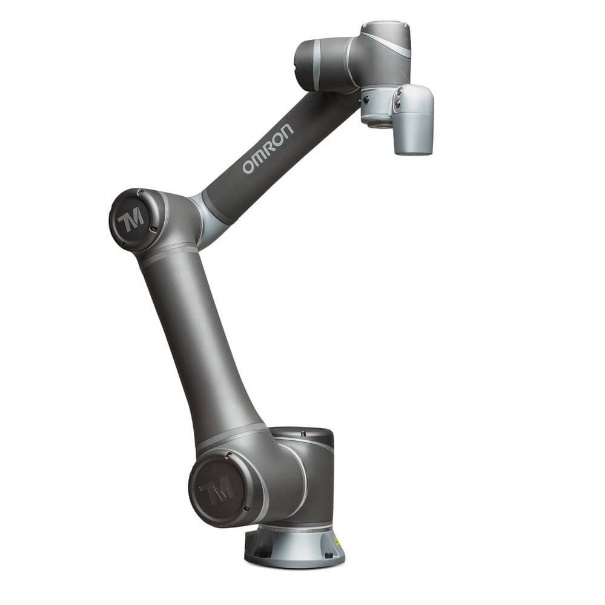
\includegraphics[width=0.6\textwidth]{images/omron.png}
    \caption{Omron TM5-900}
    \label{fig:omron}
\end{figure}

Un robot è un manipolatore riprogrammabile e multifunzionale progettato per spostare materiali, parti, strumenti o dispositivi specializzati attraverso vari movimenti programmati per l'esecuzione di una varietà di compiti. Il robot \textbf{OMRON TM5-900} è un robot industriale collaborativo (cobot) di ultima generazione, progettato per applicazioni che richiedono flessibilità, precisione e la capacità di operare in ambienti dinamici e collaborativi. È dotato di una serie di caratteristiche avanzate che lo rendono adatto a una varietà di compiti in ambienti industriali, inclusi il montaggio, il pick-and-place, e operazioni di smontaggio come quelle previste in questo progetto.

Tra le caratteristiche principali vi sono:

\begin{itemize}
    \item \textbf{Design compatto e flessibile}: Il TM5-900 è progettato per lavorare in spazi ristretti, con un braccio robotico che può essere facilmente integrato in linee di produzione esistenti senza necessitare di ampi spazi operativi. La sua flessibilità gli consente di essere facilmente usato per diverse applicazioni.
    \item \textbf{Portata e capacità di carico}: Il TM5-900 ha una capacità di carico utile fino a 5 kg, che lo rende adatto a manipolare una varietà di oggetti e strumenti, come i tessuti utilizzati in questo progetto.
    \item \textbf{Gradi di libertà (DOF)}: Il TM5-900 è dotato di 6 gradi di libertà (DOF), che gli consentono di eseguire movimenti complessi e articolati, simili a quelli di un braccio umano. Questo permette al robot di raggiungere e manipolare oggetti in spazi tridimensionali con alta precisione.
    \item \textbf{Giunti e movimenti}: Il robot è equipaggiato con giunti motorizzati, che consentono di controllare i movimenti di rotazione in modo fluido e preciso. I giunti, insieme ai sensori di forza e coppia, permettono di eseguire operazioni delicate, come il manipolamento di oggetti morbidi (ad esempio i tessuti) senza danneggiarli.
    \item \textbf{Facilità di programmazione e utilizzo}: Questo robot è dotato di un'interfaccia utente intuitiva e di software di programmazione che ne facilita l'uso anche da parte di personale non specializzato. La programmazione è resa semplice grazie alla modalità di "teaching", che consente di insegnare al robot i movimenti direttamente sul campo.
    \item \textbf{Tecnologia di sensori avanzati}: Il TM5-900 è equipaggiato con sensori di forza e coppia, che permettono di eseguire operazioni delicate con una precisione millimetrica, ideale per manipolare oggetti senza danneggiarli.
    \item \textbf{Compatibilità con ROS2}: Il robot è compatibile con il sistema ROS2, che consente di integrarlo facilmente in ambienti di simulazione come Gazebo e Unity, come previsto nel progetto. Questo permette di controllare il robot tramite comandi remoti e di simulare il suo comportamento in ambienti virtuali.
\end{itemize}

In questo progetto, il robot OMRON TM5-900 è stato scelto per la sua versatilità e capacità di manipolare oggetti come tessuti in modo preciso e sicuro. Il suo utilizzo si concentra sulla simulazione della movimentazione del robot, dove l'integrazione con ROS2 assicura una gestione ottimale della comunicazione e delle operazioni. Inoltre, l'interazione con Unity permette di visualizzare in tempo reale il comportamento del robot, monitorando e ottimizzando il suo funzionamento durante le diverse fasi del progetto.

\subsection{Stereo-Camera RealSense D435i}

\section{Software}
\textit{In questo capitolo verranno analizzati i software principali utilizzati per il progetto: Ubuntu, Robot Operating System 2, Moeveit, Gazebo e Unity. Verranno fornite una panoramica generale, informazioni sul loro utilizzo e sulle versioni adottate. Inoltre, si approfondirà l'uso del componente Cloth di Unity, che ha rivestito un ruolo centrale nella simulazione della fisica dei tessuti.}

\subsection{Ubuntu}
% \textit{Per consentire l’esecuzione degli strumenti necessari allo sviluppo del progetto, è stato necessario configurare un ambiente Linux compatibile con ROS2. A tal fine, si è scelto di utilizzare Ubuntu, installato tramite WSL (Windows Subsystem for Linux), una soluzione che permette di lavorare in ambiente Linux direttamente da un sistema operativo Windows.}

\begin{figure}[H]
    \centering
    
\includegraphics[width=0.6\textwidth]{images/ubuntu1.png}
    \caption{Logo Ubuntu}
    \label{fig:Ubuntu}
\end{figure}

Per lo sviluppo del progetto è stato utilizzato il sistema operativo \textbf{Ubuntu 22.04.5}, una distribuzione Linux molto diffusa nel campo della robotica grazie alla sua ampia compatibilità con \textbf{ROS2 (Robot Operating System 2)}.

L’installazione di Ubuntu è avvenuta tramite WSL (Windows Subsystem for Linux), una funzionalità disponibile su Windows 10 e 11 che consente di eseguire nativamente un ambiente GNU/Linux all’interno di Windows, senza dover ricorrere a una macchina virtuale o a un sistema dual boot.
In particolare, è stata utilizzata la versione WSL2, che offre prestazioni migliorate rispetto a WSL1 grazie all’integrazione di un vero e proprio kernel Linux. Questa soluzione permette di combinare la potenza e la flessibilità di Ubuntu con la praticità degli strumenti di sviluppo offerti dall’ambiente Windows.

\textbf{Di seguito, i principali passaggi eseguiti per l’installazione:} \cite{Ubuntu-install}

\begin{enumerate}
    \item Abilitazione delle funzionalità WSL e Virtual Machine Platform:
    \begin{itemize}
        \item Aprire il menu Start e cercare \textit{Windows PowerShell}.
        \item Avviare PowerShell come amministratore.
        \item Digitare il comando:
        \begin{verbatim}
wsl --install
        \end{verbatim}
        Questo comando installa WSL2 come versione predefinita. Al termine dell’installazione, sarà necessario riavviare il computer.
    \end{itemize}
    \item Installazione di Ubuntu 22.04
        \begin{itemize}
            \item Dopo aver abilitato WSL2, è possibile installare Ubuntu digitando:
            \begin{verbatim}
    wsl --install -d Ubuntu-22.04
            \end{verbatim}
        \end{itemize}
    Al termine dell’installazione, sarà necessario riavviare il computer.


    \item Configurazione iniziale:
        \begin{itemize}
            \item Al primo avvio, verrà richiesto di creare un utente e una password Linux.
            \item Infine, è consigliato aggiornare i pacchetti eseguendo:
            \begin{verbatim}
        sudo apt update && sudo apt upgrade
            \end{verbatim}
        \end{itemize}
\end{enumerate}



Questa configurazione ha permesso l’installazione di ROS2 e l’integrazione con librerie e strumenti specifici per la robotica, mantenendo una buona compatibilità con gli altri software utilizzati nel progetto, come Unity e Gazebo.





\subsection{Robot Operating System 2}

\begin{figure}[H]
    \centering
    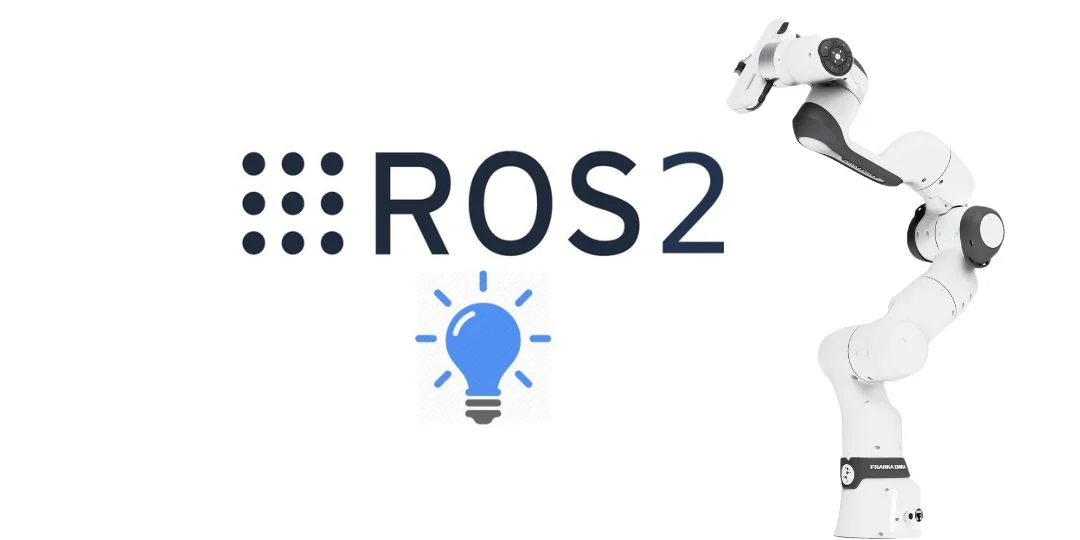
\includegraphics[width=0.6\textwidth]{images/ROS2.png}
    \caption{Logo ROS2}
    \label{fig:ROS2}
\end{figure}

\textbf{ROS 2} (Robot Operating System 2) \cite{ROS2} è un framework open-source per lo sviluppo di applicazioni robotiche. Fornisce una serie di strumenti, librerie e convenzioni per facilitare la comunicazione tra i componenti software di un sistema robotico. ROS 2 è progettato per migliorare la scalabilità, la sicurezza e la compatibilità con i sistemi distribuiti rispetto al suo predecessore, ROS 1. Il suo utilizzo è diffuso in ricerca e industria per il controllo di robot mobili, bracci robotici e veicoli autonomi.
In questo progetto, ROS 2 è stato utilizzato per gestire la comunicazione tra il robot simulato in Unity e i componenti di controllo. ROS 2 permette lo scambio di messaggi tra i nodi, abilitando il controllo del robot da Unity e viceversa. In particolare, il framework ha permesso l'integrazione con il sistema di simulazione, la gestione delle traiettorie e il controllo dei giunti del manipolatore.
Inizialmente, il progetto è stato avviato con ROS 2 Jazzy, ma si sono riscontrati diversi problemi di compatibilità e instabilità, in particolare con l'integrazione del ROS-TCP Connector per Unity. Per questo motivo, è stato deciso di passare a ROS 2 Humble, una versione più stabile e ampiamente supportata, che ha garantito una migliore compatibilità con gli strumenti di sviluppo utilizzati.

\subsection{Moveit}
\label{sec:moveit}
\begin{figure}[H]
    \centering
    
\includegraphics[width=0.6\textwidth]{images/moveit.png}
    \caption{Logo Moveit}
    \label{fig:moveit}
\end{figure}
\textbf{MoveIt} \cite{Moveit} \cite{Moveit_install} è una delle librerie più utilizzate per la pianificazione del movimento in ROS. Consente di controllare bracci robotici, eseguire pianificazioni di traiettoria, gestire collisioni e implementare strategie di manipolazione avanzate. Grazie alla sua integrazione con ROS 2, MoveIt permette di generare e simulare movimenti in modo efficiente, facilitando l'implementazione di algoritmi di pianificazione e controllo.

MoveIt utilizza il modello del robot descritto tramite URDF per comprendere la struttura cinematica del sistema e genera automaticamente il corrispettivo SRDF (Semantic Robot Description Format) contenente la generazione di movimenti validi evitando collisioni. Il suo framework è composto da diversi moduli, tra cui:
\begin{itemize}
    \item Motion Planning: per la generazione di traiettorie.
    \item Collision Checking: per evitare urti tra il robot e l'ambiente.
    \item Kinematic Solvers: per calcolare i movimenti articolari necessari a raggiungere una determinata posizione.
    \item Trajectory Execution: per inviare comandi al robot fisico o alla simulazione.
\end{itemize}

Nel nostro progetto, MoveIt è stato utilizzato per pianificare e simulare i movimenti del manipolatore Omron TM5-900. Tramite il MoveIt Setup Assistant è stato possibile definire i gruppi cinematici, i giunti controllabili e le geometrie di collisione.

MoveIt è stato integrato con ROS 2 Humble tramite la versione Moveit2 e tramite questa libreria sono state svolte le seguenti operazioni:
\begin{itemize}
    \item Creazione del file SRDF tramite MoveIt Setup Assistant.

    \item Definizione dei controller nel file $ros2\_controllers.yaml$.

    \item Definizione delle pose iniziali e finali del robot.

    \item Invio delle traiettorie a Unity per visualizzare e simulare il movimento del robot in un contesto 3D realistico.
\end{itemize}

Alla sezione \ref{sec:moveit_setup_assistant} è presente una descrizione dettagliata dei passaggi svolti con il MoveIt Setup Assistant per la creazione del file SRDF e la definizione dei controller.
\subsection{Gazebo}

\subsubsection*{Modellazione e simulazione robotica in ROS 2 con URDF, XACRO, SDF e Gazebo}

In ambiente \textbf{ROS 2}, la modellazione e la simulazione robotica si basano su un insieme di strumenti e formati standardizzati che consentono la rappresentazione dettagliata dei robot e del mondo simulato. Il formato \textbf{URDF} (Unified Robot Description Format) viene utilizzato per descrivere la struttura fisica e cinematica di un robot, includendo elementi come i \textit{link} (parti rigide), le \textit{joint} (articolazioni mobili), le geometrie visuali e di collisione, e le proprietà fisiche quali massa, inerzia e materiali. URDF è nativamente supportato da ROS 2 ed è lo standard di riferimento per la descrizione dei modelli robotici.

Per migliorare la modularità e la riusabilità del codice, viene spesso impiegata l’estensione \textbf{XACRO} (XML Macros), che consente di definire macro, parametri e inclusioni di file esterni. XACRO permette una gestione più efficiente di modelli complessi, sebbene sia necessario convertirne i file in formato URDF standard prima dell’utilizzo in Gazebo, tramite un semplice comando da terminale:

\begin{quote}
\texttt{xacro my\_robot.urdf.xacro > my\_robot.urdf}
\end{quote}

La simulazione fisica e visuale viene gestita da \textbf{Gazebo}, un simulatore open source sviluppato originariamente presso la University of Southern California e successivamente mantenuto dalla \textit{Open Source Robotics Foundation}. Gazebo permette la simulazione realistica dell’interazione tra robot e ambiente, includendo dinamiche fisiche, sensori virtuali, rendering 3D e supporto a plugin personalizzati.

Per la descrizione dell’ambiente simulato, Gazebo utilizza un formato nativo denominato \textbf{SDF} (Simulation Description Format), più completo rispetto a URDF e adatto a rappresentare terreni, luci, oggetti dinamici o statici, proprietà ambientali e plugin. Nell’ambito ROS 2, l’approccio più comune consiste nell’utilizzare URDF (o XACRO) per la descrizione del robot e SDF per la definizione del mondo simulativo.

Il collegamento tra ROS 2 e Gazebo è garantito dal pacchetto \texttt{gazebo\_ros}, che funge da interfaccia tra i due ambienti. Questo bridge consente l’integrazione di modelli URDF/XACRO nella simulazione, la pubblicazione dei dati sensoriali simulati su topic ROS 2, l’interazione con i robot tramite comandi ROS e la sincronizzazione del tempo simulato con il clock del sistema ROS. L’adozione combinata di URDF/XACRO, SDF, Gazebo e \texttt{gazebo\_ros} rappresenta dunque una soluzione completa e flessibile per lo sviluppo, il test e la validazione di sistemi robotici complessi all’interno di ambienti simulati.



\subsection{Unity e UnityHUB}

\begin{figure}[H]
    \centering
    
\includegraphics[width=0.6\textwidth]{images/UNITY.jpg}
    \caption{Logo Unity}
    \label{fig:UNITY}
\end{figure}

\textbf{Unity} \cite{Unity} è un motore di gioco e simulazione ampiamente utilizzato per la creazione di ambienti interattivi in tempo reale. Sebbene sia nato per lo sviluppo di videogiochi, il suo utilizzo si è esteso ad applicazioni di simulazione, robotica, realtà virtuale e aumentata. Unity permette di creare ambienti 3D realistici e interattivi grazie al suo motore grafico avanzato e alle sue funzionalità di scripting basate su C\#.
In questo progetto, Unity è stato utilizzato come ambiente di simulazione per il robot. Grazie alla sua compatibilità con ROS2 tramite il ROS-TCP Connector, Unity ha permesso di visualizzare il robot, simulare i suoi movimenti e interagire con l'ambiente circostante. Il motore fisico di Unity è stato sfruttato soprattutto per replicare le dinamiche fisiche della maglietta, garantendo una simulazione più realistica delle interazioni tra un indumento e gli oggetti della scena.
Per lo sviluppo del progetto, abbiamo utilizzato Unity 6, la versione più recente al momento di sviluppo del progetto.

\subsection{Strumento Cloth di Unity}
Il sistema \textbf{Cloth di Unity} offre una soluzione basata sulla fisica per simulare tessuti e materiali flessibili all'interno di ambienti 3D. Sebbene sia stato progettato principalmente per rappresentare abbigliamento su personaggi, può essere utilizzato anche per altri scopi, come bandiere, tende o qualsiasi altro oggetto che richieda una simulazione realistica del comportamento dei tessuti\cite{ManualCloth}.
In questo progetto, il componente Cloth riveste un ruolo centrale, poiché il compito finale prevede che l'indumento manipolato dal robot presenti una fisica il più possibile realistica, simulando accuratamente il comportamento del tessuto. A tal fine, sono stati forniti tre file principali relativi a una maglietta: un file \textbf{OBJ}, un file \textbf{FBX} e un file \textbf{Collada}. 
L'analisi di questi file ha permesso di ottenere informazioni utili riguardo al formato da utilizzare e alle caratteristiche della mesh per applicare efficacemente il componente Cloth.
\newline
Tra la documentazione di Unity è possibile trovare anche quella relativa al componente Cloth e in seguito verranno riassunti i passaggi fondamentali per utilizzarlo al meglio.
Per implementare una simulazione di tessuto in Unity, è necessario aggiungere il componente Cloth a un oggetto mesh. Ecco i passaggi fondamentali:
\begin{itemize}
    \item \textbf{Preparazione della Mesh}: è importante assicurarsi che l'oggetto a cui si desidera applicare il tessuto abbia una mesh adeguata, e quindi, come visto in precedenza, anche un numero adeguato di poligoni della mesh.
    
    \item \textbf{Aggiunta del Componente}: una volta importato il file su Unity è sufficiente selezionare l'oggetto nella gerarchia di Unity e, nel pannello Inspector, cliccare su "Add Component", selezionare "Physics" e poi "Cloth" dalla lista dei componenti disponibili.

    \item \textbf{Configurazione}: Una volta aggiunto il componente, sarà possibile modificare vari parametri per ottenere una simulazione personalizzata e accurata.
\end{itemize}

Affinchè la maglietta abbia una movimentazione guidata dalla fisica, deve chiaramente avere una parte della maglietta fissata e che quindi non è soggetta alla gravità. Questi su Unity vengono chiamati "Cloth Constraint" e quindi "vincoli del Cloth".
Di seguito una descrizione dei passaggi per applicarli correttamente alla maglietta:
\begin{enumerate}
    \item sul componente Cloth si clicca su "Edit Cloth Constraint" come possiamo vedere dalla figura \ref{fig:cloth_constraints}
    \begin{figure}[h!]
        \centering
        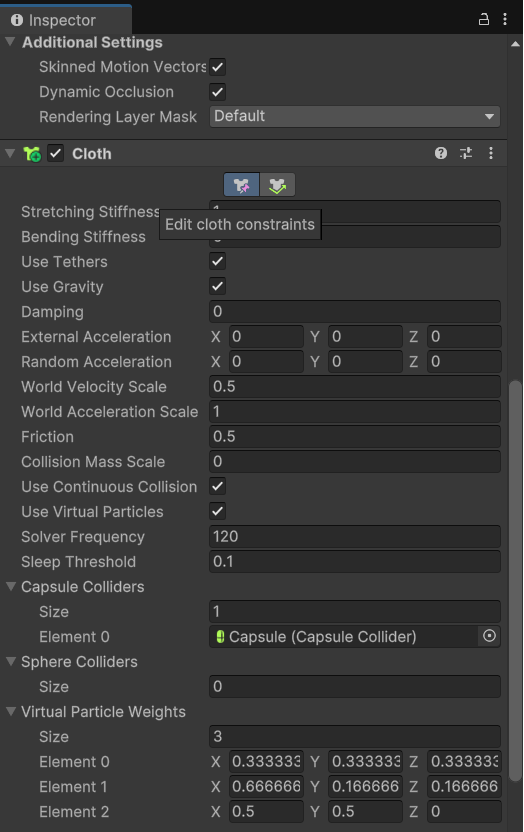
\includegraphics[width=0.3\textwidth]{images/cloth_constraints.PNG}
        \caption{Schermata Unity per l'applicazione dei vincoli}
        \label{fig:cloth_constraints}
    \end{figure}
    \item successivamente si aprirà una schermata che permetterà di selezionare (tramite "Select") oppure colorare (tramite "Paint") le parti che saranno vincolate e quindi rimarranno maggiormente rigide. E' importante specificare una distanza minima nel parametro "Max Distance", in figura \ref{fig:cloth_constraints_2} è stato assegnato il valore 0.2 ed ha permesso un buon risultato.
    \begin{figure}[h!]
        \centering
        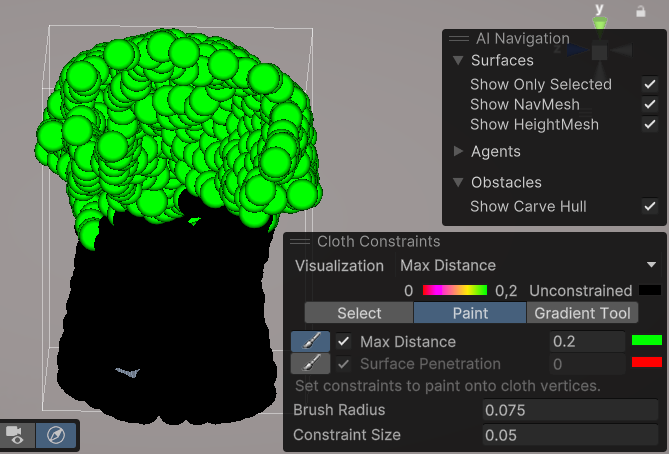
\includegraphics[width=0.5\textwidth]{images/cloth_constraints_2.PNG}
        \caption{Schermata Unity per la selezione delle parti della mesh a cui applicare i vincoli}
        \label{fig:cloth_constraints_2}
    \end{figure}
\end{enumerate}



Infine una descrizione delle principali proprietà del componente Cloth e di come sono state utilizzate nell'implementazione del tessuto realistico della maglietta:
\begin{itemize}
    \item \textbf{Stretching Stiffness}: Determina la resistenza del tessuto all'allungamento. Valori più alti rendono il tessuto meno incline a estendersi. Un parametro accettabile per la maglietta è risultato compreso tra 0,5 e 0,7.

    \item \textbf{Bending Stiffness}: Controlla la rigidità alla flessione del tessuto. Un valore elevato riduce la capacità del tessuto di piegarsi. Un parametro accettabile per la maglietta è risultato compreso tra 0,7 e 0,9.

    
    \item \textbf{Use Tethers}: Applica vincoli che aiutano a prevenire che le particelle mobili del tessuto si allontanino troppo da quelle fisse, riducendo l'eccessiva elasticità.
    
    \item \textbf{Use Gravity}: Indica se la gravità deve influenzare il tessuto. Da applicare nel caso in cui si voglia vedere una movimentazione fisica della maglietta e condizionata dalla gravità.
    
    \item \textbf{Damping}: Coefficiente che determina quanto velocemente il movimento del tessuto si smorza nel tempo.  Un parametro accettabile per la maglietta è risultato compreso tra 0,2 e 0,4.
    
    \item \textbf{External Acceleration}: Applica un'accelerazione costante esterna al tessuto, utile per simulare effetti come il vento.
    
    \item \textbf{Random Acceleration}: Introduce un'accelerazione casuale al tessuto, aggiungendo variazioni imprevedibili nel movimento.
    
    \item \textbf{World Velocity Scale}: Determina quanto il movimento in spazio globale dell'oggetto influisce sui vertici del tessuto.
    
    \item \textbf{World Acceleration Scale}: Controlla l'influenza dell'accelerazione globale dell'oggetto sui vertici del tessuto.
    
    \item \textbf{Friction}: Imposta il coefficiente di attrito del tessuto durante le collisioni.  Un parametro accettabile per la maglietta è risultato compreso tra 0,5 e 0,7.
    
    \item \textbf{Collision Mass Scale}: Determina l'incremento di massa delle particelle durante le collisioni.
    
    \item \textbf{Use Continuous Collision}: Abilita la collisione continua per migliorare la stabilità delle interazioni.
    
    \item \textbf{Use Virtual Particles}: Aggiunge particelle virtuali per migliorare la stabilità delle collisioni.
    
    \item \textbf{Solver Frequency}: Specifica il numero di iterazioni del solver per secondo, influenzando la precisione della simulazione. Un parametro accettabile per la maglietta è risultato 60 Hz.
    
    \item \textbf{Sleep Threshold}: Definisce la soglia sotto la quale il tessuto entra in stato di "sonno", interrompendo la simulazione fino a nuove interazioni. Un parametro accettabile per la maglietta è risultato 0,1. 
    
    \item \textbf{Capsule Colliders}: Array di collisori a capsula con cui il tessuto può interagire.
    
    \item \textbf{Sphere Colliders}: Array di coppie di collisori sferici con cui il tessuto può interagire.
\end{itemize}



% \section{Componente1}
% \section{Componente2}
% \section{Schema dei collegamenti}
% Inserire uno schema dei collegamenti analogo a quello in Figura \ref{fig:schema}. Si suggerisce per lo scopo di usare il software "draw.io". Nello schema riportare tutti i collegamenti tra i componenti, specificando quale pin di un componente1 si collega con quale pin di un componente2 (per la maggior parte dei collegamenti dovete cioè avere una linea con 2 label). \\
% Inserire anche una descrizione testuale dello schema.

% \begin{figure}[H]
% \centering
% 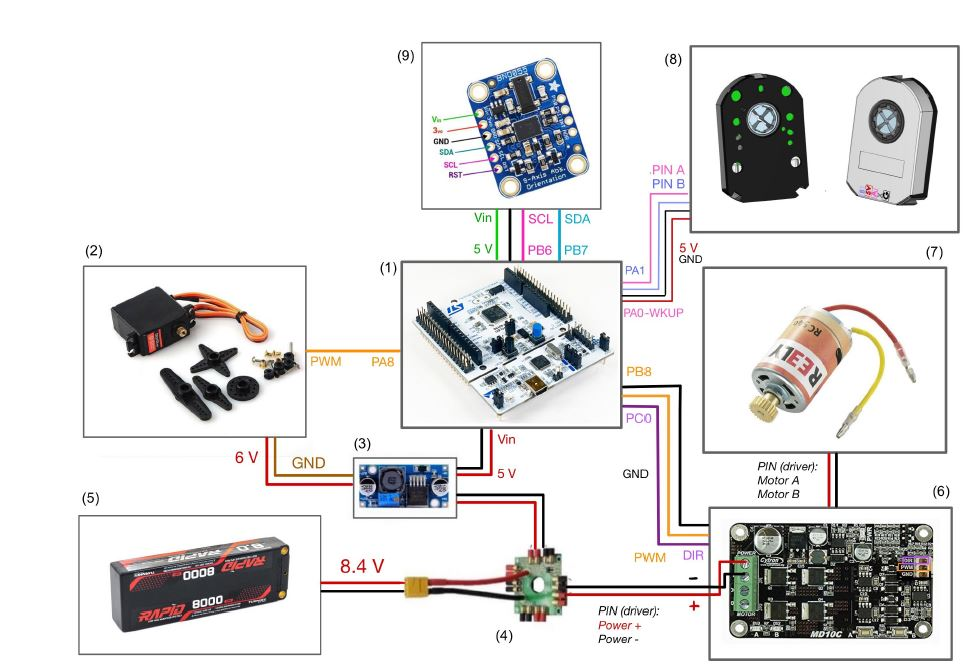
\includegraphics[width=0.8\textwidth,keepaspectratio]{figures/Schema.JPG}
% \caption{Schema dei collegamenti}
% \label{fig:schema}
% \end{figure}

\section{Predisposizione dei Software nel PC}
\textit{In questo capitolo viene presentata la configurazione dell'ambiente di lavoro adottato per lo sviluppo del progetto, con particolare attenzione alle versioni e alle modalità di integrazione dei principali software utilizzati: Ubuntu, ROS2, Gazebo, Unity (insieme a Unity Hub) e MoveIt2.}

Per la parte robotica e di simulazione, è stato scelto di adottare \textbf{Ubuntu 22.04} installato tramite una macchina virtuale WSL2, in quanto offre un ambiente stabile e supportato ufficialmente per lo sviluppo con \textbf{ROS2 Humble} e \textbf{MoveIt2}. ROS2 Humble è stato selezionato per la sua affidabilità e le migliorate capacità di integrazione, che hanno risolto i problemi riscontrati con precedenti versioni (come Jazzy).\textbf{Gazebo Fortress}, la cui scelta della versione è dovuta alla compatibilità con ROS2\cite{Gazebo-ROS2}, garantisce simulazioni avanzate e un'elevata accuratezza nella riproduzione delle dinamiche robotiche, tuttavia non ha un ruolo centrale nel progetto in quanto non è possibile applicare la fisica ai tessuti come in Unity.

Parallelamente, per lo sviluppo dell'ambiente 3D e della visualizzazione in tempo reale, si è mantenuto \textbf{Unity 6}(ultima versione) su Windows, supportato da \textbf{Unity Hub} che permette una gestione semplificata dei vari progetti Unity. La scelta di utilizzare Windows come sistema operativo per Unity è motivata dalla sua eccellente compatibilità con gli strumenti grafici e i driver necessari per un'interfaccia utente fluida e performante, in quanto Unity è un software nativo Windows. La comunicazione tra l'ambiente robotico gestito tramite Ubuntu e quello grafico su Windows è resa possibile attraverso il ROS-TCP Connector, che funge da ponte tra le due piattaforme, garantendo lo scambio efficiente dei dati.

Questa configurazione ibrida, che sfrutta al massimo le potenzialità di ogni sistema operativo e software specifico, consente di ottimizzare sia le prestazioni delle simulazioni che l'interattività dell'interfaccia grafica, contribuendo a rendere il progetto complessivamente robusto e flessibile.
\section{Interfacciamento ROS2-Unity}

\textit{Il capitolo "Interfacciamento ros2-Unity" si propone di illustrare come integrare in maniera efficace ROS2 con l’ambiente grafico e simulativo offerto da Unity, al fine di realizzare una piattaforma in grado di gestire in tempo reale sia la simulazione fisica che la comunicazione dei dati. In particolare, saranno mostrati il ROS-TCP Connector e il ROS-TCP Endpoint per lo scambio di messaggi tra ROS2 e Unity, nonché l'URDF Importer per la corretta rappresentazione del robot all'interno di Unity.}

\subsection{ROS-TCP Connector \& ROS-TCP Endpoint}
Unity Technologies fornisce un pacchetto che consente di integrare ROS2 con Unity, facilitando la comunicazione tra i due ambienti. Questo pacchetto è composto da due nodi principali e complementari tra loro: il \textbf{ROS-TCP Connector} e il \textbf{ROS-TCP Endpoint}.
In particolare il \textbf{ROS-TCP Connector} è un pacchetto Unity che consente di inviare e ricevere messaggi tra Unity e ROS2, mentre il \textbf{ROS-TCP Endpoint} è un nodo ROS2 che funge da server TCP, ascoltando le connessioni in entrata da Unity e gestendo lo scambio di messaggi tra i due ambienti.
\newline
% Il \textbf{ROS-TCP Connector} è un pacchetto sviluppato da Unity Technologies che permette di mettere in comunicazione ROS2 e Unity attraverso una connessione TCP. Questa integrazione è fondamentale perché consente di inviare e ricevere messaggi tra i due ambienti, facilitando lo sviluppo e la simulazione di robot. Grazie a questo pacchetto, Unity diventa un ambiente in cui è possibile visualizzare i dati provenienti da ROS2, testare il controllo e verificare il comportamento del robot in scenari simulati prima di passare alla fase di implementazione su un sistema reale.

Il pacchetto ROS-TCP Connector include:

\begin{itemize}
    \item \textbf{ROS-TCP Connector}: permette l’invio e la ricezione di messaggi tra Unity e ROS2.
    \item \textbf{VISUALIZATIONS PACKAGE}: utile per la visualizzazione dei messaggi in entrata e in uscita nella scena di Unity, facilitando il debug e l'analisi dei dati.
\end{itemize}

Inoltre, il pacchetto offre diverse funzionalità:

\begin{itemize}
    \item \textbf{ROSConnection}: gestisce l’intero processo di comunicazione tra Unity e ROS2.
    \item \textbf{Message Generation}: permette di generare automaticamente classi in C\# che rappresentano i messaggi ROS2, facilitando l’interazione tra i due ambienti.
    \item \textbf{Visualizations}: un set di API e configurazioni predefinite per rappresentare le informazioni scambiate.
    \item \textbf{ROSGeometry}: una serie di estensioni utili per la conversione delle geometrie tra Unity e altri sistemi che semplificano la compatibilità tra gli ambienti di simulazione.
\end{itemize}

Per utilizzare il ROS-TCP Connector, è necessario installarlo all’interno di Unity e configurarlo correttamente affinché possa dialogare con ROS2.

Il pacchetto è disponibile su GitHub e può essere importato in Unity tramite il Package Manager. Ecco come fare:

\begin{itemize}
    \item Aprire Unity e accedere al menu "Window", poi selezionare "Package Manager".
    \begin{figure}[h]
        \centering
        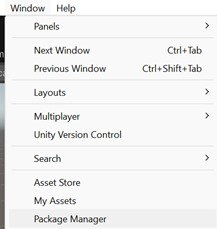
\includegraphics[width=0.4\textwidth]{images/rostcp.jpg}
        \caption{Package Manager in Unity}
        \label{fig:rostcp}
    \end{figure}
    
    \item Nella finestra del Package Manager, cliccare sul pulsante “+” in alto a sinistra e selezionare "Add package from git URL...".
    \begin{figure}[h]
        \centering
        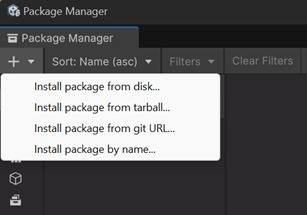
\includegraphics[width=0.4\textwidth]{images/rostcp1.jpg}
        \caption{Package Manager in Unity}
        \label{fig:rostcp1}
    \end{figure}

    \item Inserire l’URL del pacchetto da installare:
    \begin{itemize}
        \item \textbf{ROS-TCP Connector}: 
        \url{https://github.com/Unity-Technologies/ROS-TCP-Connector.git?path=/com.unity.robotics.ros-tcp-connector}
        % \item \textbf{Visualizations Package}: 
        % \url{https://github.com/Unity-Technologies/ROS-TCP-Connector.git?path=/com.unity.robotics.visualizations}
    \end{itemize}
    
    In alternativa, se si ha una copia locale del pacchetto, è possibile installarlo seguendo la guida ufficiale di Unity per l’installazione di pacchetti locali.
\end{itemize}

Dopo aver installato il pacchetto, è necessario configurarlo per far sì che possa comunicare con ROS2. Questo passaggio è essenziale per garantire che Unity e ROS2 possano scambiarsi dati senza problemi:

% Dopo aver caricato l’oggetto, per configurare la comunicazione, bisogna:

\begin{itemize}
    \item Accedere al menu "Robotics" e selezionare "ROS Settings".
    \begin{figure}[H]
        \centering
        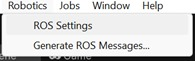
\includegraphics[width=0.4\textwidth]{images/rostcp2.jpg}
        \caption{Menu "Robotics" e "ROS Settings"}
        \label{fig:rostcp2}
    \end{figure}
    
    \item Nel campo "ROS IP Address", inserire l'indirizzo IP della macchina su cui è in esecuzione ROS2.
    \begin{figure}[H]
        \centering
        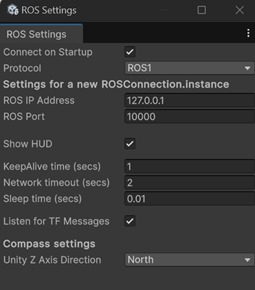
\includegraphics[width=0.4\textwidth]{images/rostcp4.jpg}
        \caption{Configurazione dell'indirizzo IP di ROS2}
        \label{fig:rostcp4}
    \end{figure}
\end{itemize}

Per reperire l'indirizzo IP di ROS (ROS IP Address) sulla macchina con WSL, è sufficiente aprire un terminale e digitare:

\begin{verbatim}
hostname -I
\end{verbatim}

Ora lato Unity la comunicazione è pronta, quindi procediamo con l'installazione e la configurazione del \textbf{ROS-TCP Endpoint} lato ROS2.
Per utilizzarlo, è necessario installarlo all'interno del proprio workspace ROS2, clonando la repository tramite il comando: \cite{Repository-ROS-TCP-Endpoint}
\begin{verbatim}
    git clone https://github.com/Unity-Technologies/ROS-TCP-Endpoint.git
\end{verbatim}

    % \item \textbf{Compilare il workspace}: \texttt{cd ~/tuo\_workspace}
    % \begin{verbatim}
    % colcon build --symlink-install
    % source install/setup.bash
    % \end{verbatim}

Dopo aver completato l’installazione e la configurazione, Unity sarà in grado di comunicare con ROS2 attraverso il protocollo TCP. Questo avviene tramite due modalità principali:
    
\begin{itemize}
    \item \textbf{Pubblicazione di Messaggi}: Unity può inviare dati a ROS2 utilizzando il componente \texttt{ROSPublisher}.
    \item \textbf{Sottoscrizione di Messaggi}: Unity può ricevere dati da ROS2 grazie al componente \texttt{ROSSubscriber}.
\end{itemize}

A questo punto, per verificare che le installazioni e le configurazioni siano avvenute con successo è possibile seguire un breve tutorial per testare la connessione tra Unity e ROS2.
In particolare l'obiettivo sarà quello di inviare le coordinate di un oggetto di Unity a ROS2 tramite un Publisher e ricevere le coordinate di un oggetto di ROS2 in Unity tramite un Subscriber, il link è in bibliografia.\cite{Test-Connessione-ROS-Unity}

Tuttavia, seguono i comandi generali che saranno poi nuovamente riproposti alla sezione \ref{cap:Test}.

Inizialmente, è necessario avviare il nodo \texttt{ros\_tcp\_endpoint} all’interno di ROS2. Questo nodo funge da intermediario e garantisce che i messaggi possano fluire correttamente tra i due sistemi.
    
Per avviare il nodo \textbf{ros\_tcp\_endpoint}, bisogna eseguire il comando:

\begin{verbatim}
    ros2 run ros_tcp_endpoint default_server_endpoint --ros-args -p ROS_IP:=YOUR_IP
\end{verbatim}

Dove per conoscere l'indirizzo IP del proprio computer è possibile utilizzare il comando: 
\begin{verbatim}
    hostname -I
\end{verbatim}

In questo modo si avvia il server che ascolta sulla porta TCP (di default 10000) per ricevere le connessioni da Unity.

A questo punto, se nella Scena di Unity è presente un Publisher o un Subscriber configurato correttamente, Unity tenterà di connettersi al nodo \textbf{ros\_tcp\_endpoint} e inizierà a inviare o ricevere messaggi.
In particolare una volta avviata la simulazione in Unity dovremmo vedere le due frecce rosse come mostrato in figura \ref{fig:test_connessione_1}.

\begin{figure}[H]
    \centering
    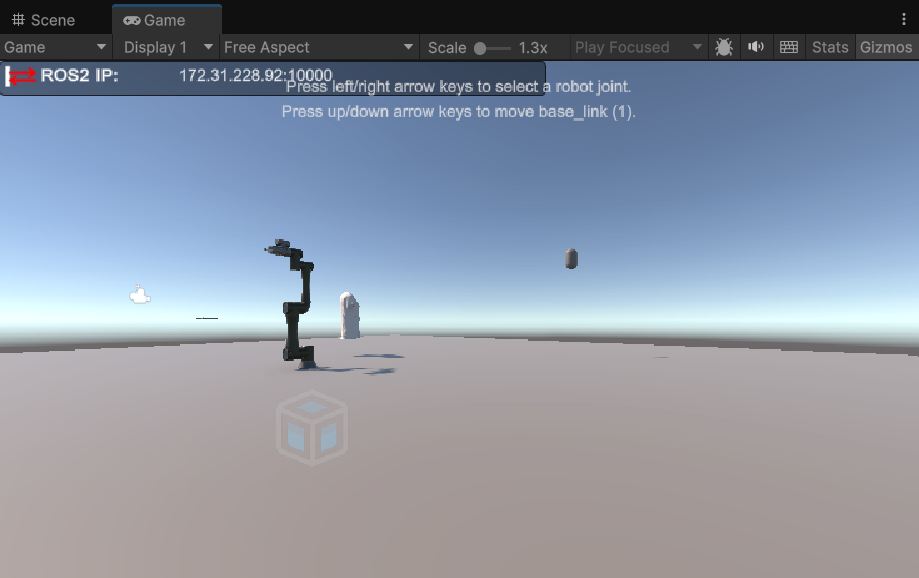
\includegraphics[width=0.6\textwidth]{images/test_connessione_1.PNG}
    \caption{Test della connessione una volta avviata la simulazione}
    \label{fig:test_connessione_1}
\end{figure}

Successivamente, una volta che è stato avviato il ROS-TCP-Endpoint le frecce cambieranno colore in blu, indicando che la connessione è stata stabilita con successo, come mostrato in figura \ref{fig:test_connessione_2}.

\begin{figure}[H]
    \centering
    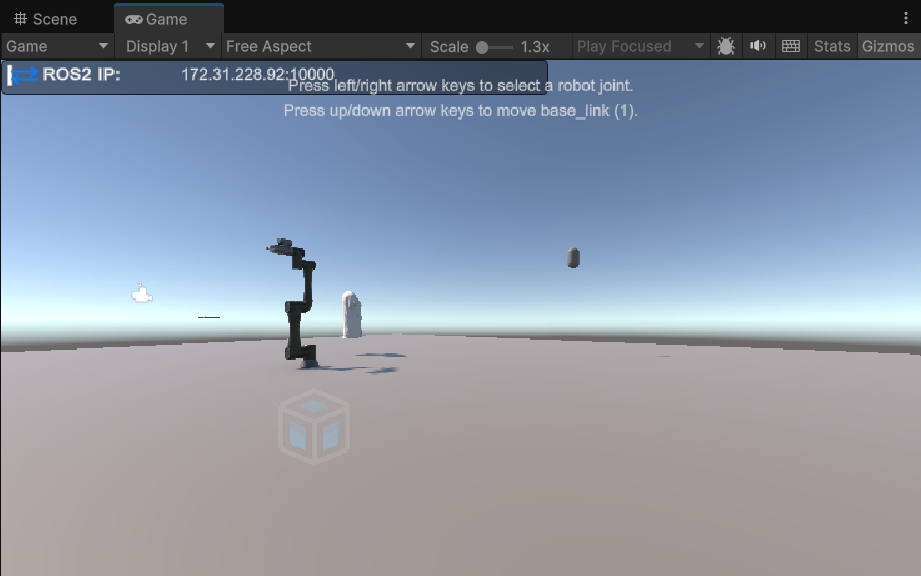
\includegraphics[width=0.6\textwidth]{images/test_connessione_2.PNG}
    \caption{Test della connessione dopo aver avviato il ROS-TCP-Endpoint}
    \label{fig:test_connessione_2}
\end{figure}
% Per assicurarsi che il nodo sia in esecuzione, è possibile utilizzare il comando: \begin{verbatim}
% ros2 node list
% \end{verbatim}

% In questo modo il nodo \textbf{/ros\_tcp\_endpoint\_node} dovrebbe essere visibile nella lista.

\subsection{URDF Importer}
\label{sec:urdf_importer}
L'\textbf{URDF Importer} \cite{URDF-Importer} di Unity è uno strumento che permette di importare file URDF (Unified Robot Description Format) direttamente in Unity, consentendo così di visualizzare e interagire con modelli robotici 3D all'interno dell'ambiente di simulazione. Questo strumento risulta particolarmente utile nel progetto perché permette di integrare ROS 2 e Unity tramite il file URDF fortemente utilizzato in robotica, inoltre semplifica la gestione della cinematica e della fisica dei robot senza dover ricostruire manualmente i modelli.

Il formato URDF è ampiamente utilizzato nel mondo della robotica per descrivere la struttura dei robot, inclusi i links, i joints, i materiali e i sensori. L'URDF Importer converte questi modelli in GameObjects di Unity, mantenendo la gerarchia dei componenti e assegnando i giunti come oggetti fisici controllabili.

Nel nostro progetto, il robot utilizzato è un Omron TM5-900, un braccio robotico con sei gradi di libertà. Il modello URDF di questo robot contiene:
\begin{itemize}
    \item Link per ogni segmento del braccio, dalla base all'end-effector.
    \item Joints di tipo rotoidale che consentono il movimento.
    \item Materiali per rappresentare visivamente il robot in Unity.
    \item Collisioni e inerzia, che permettono una simulazione fisica realistica.
\end{itemize}

L'importazione di questo URDF in Unity è essenziale per poterlo visualizzare correttamente e per interagire con esso tramite ROS 2.

Per importare installare lo strumento URDF Importer è possibile seguire i seguenti passaggi:
\begin{itemize}
    \item Cliccare su "Window" poi "Package Manager"
    \begin{figure}[H]
        \centering
        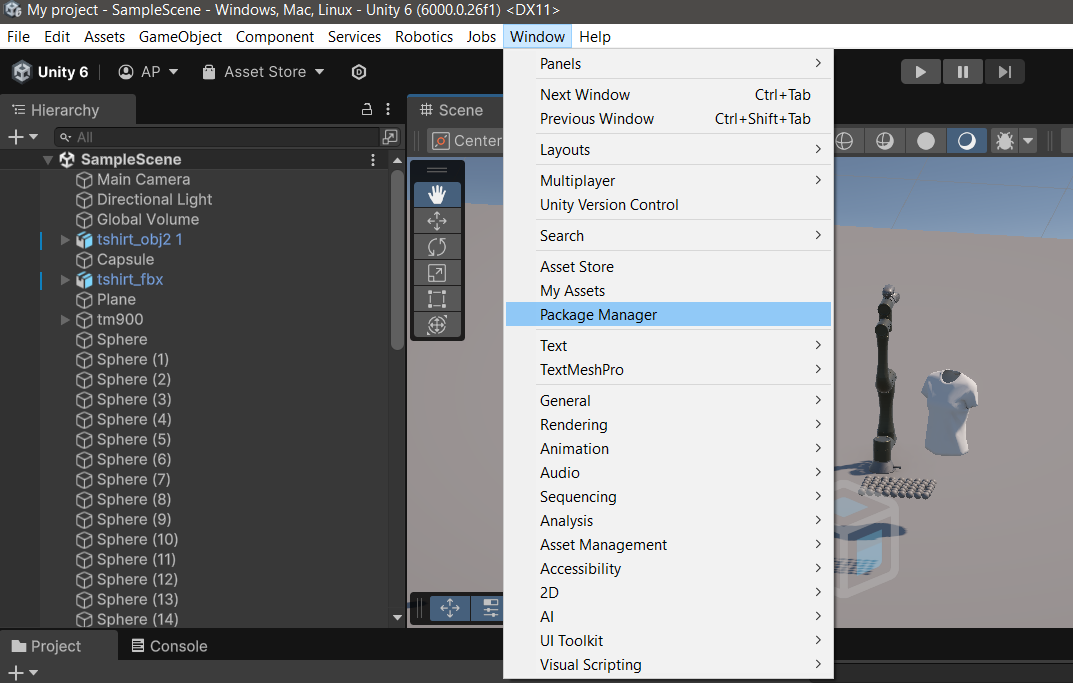
\includegraphics[width=0.4\textwidth]{images/URDF_Importer_1.png}
        \caption{URDF Importer Tutorial}
        \label{fig:URDF_Importer_1}
    \end{figure}
    \item Cliccare su "+" e selezionare "Add package from git URL..."
    \begin{figure}[H]
        \centering
        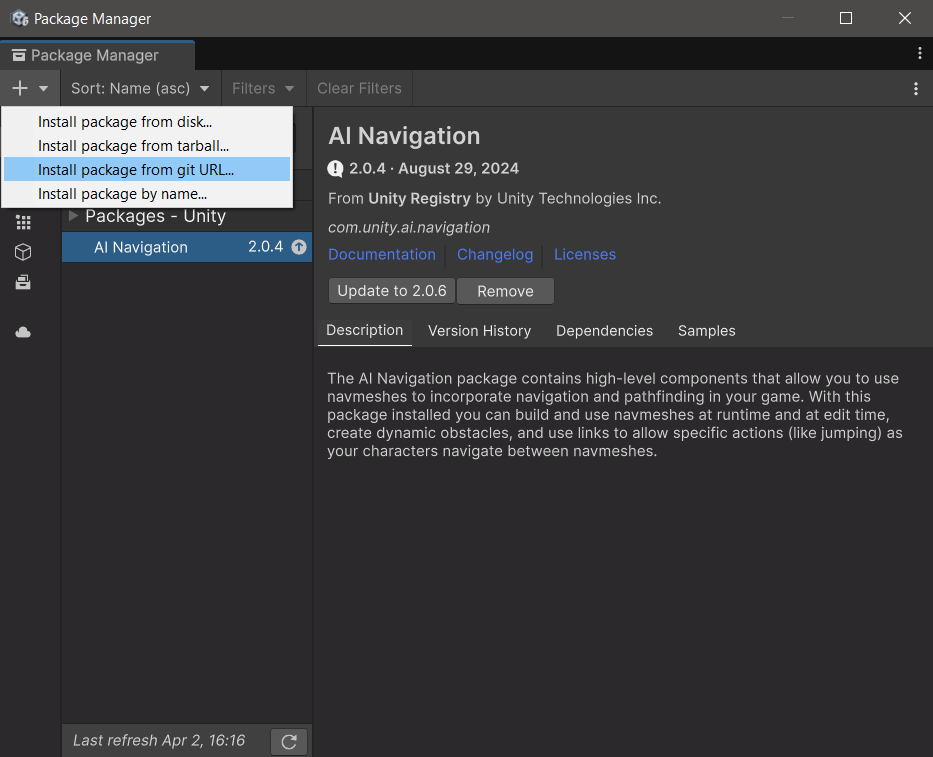
\includegraphics[width=0.4\textwidth]{images/URDF_Importer_2.png}
        \caption{URDF Importer Tutorial}
        \label{fig:URDF_Importer_2}
    \end{figure}
    \item Inserire il seguente URL della repository: 
    \url{https://github.com/Unity-Technologies/URDF-Importer.git} e cliccare "install" per avviare l'installazione
    \begin{figure}[H]
        \centering
        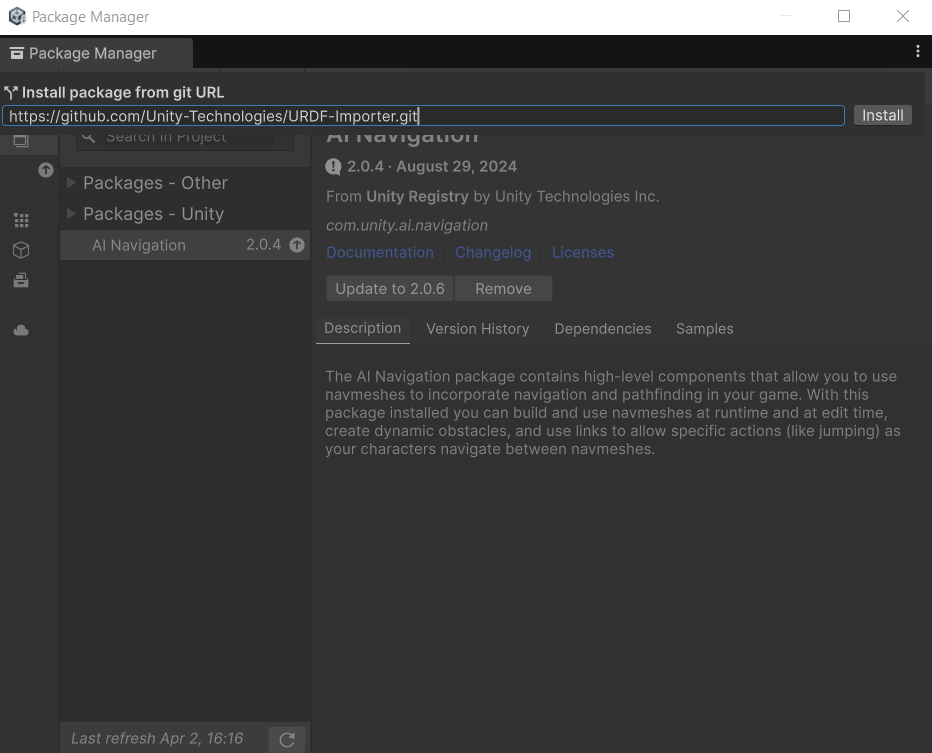
\includegraphics[width=0.4\textwidth]{images/URDF_Importer_3.png}
        \caption{URDF Importer Tutorial}
        \label{fig:URDF_Importer_3}
    \end{figure}
\end{itemize}

Per importare il modello URDF su Unity invece:
\begin{itemize}
    \item Importare il file URDF e le varie mesh sia visual che collision nella cartella "Assets" del progetto Unity
    \begin{figure}[H]
        \centering
        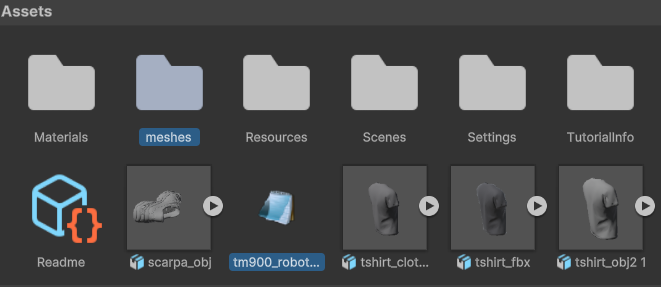
\includegraphics[width=0.5\textwidth]{images/URDF_Importer_4.png}
        \caption{URDF Importer Tutorial}
        \label{fig:URDF_Importer_4}
    \end{figure}
    \item Verificare che i vari path delle mesh all'interno del file URDF siano del tipo ""package://path/delle/meshes" come mostrato in figura \ref{fig:URDF_Importer_5}
    \begin{figure}[H]
        \centering
        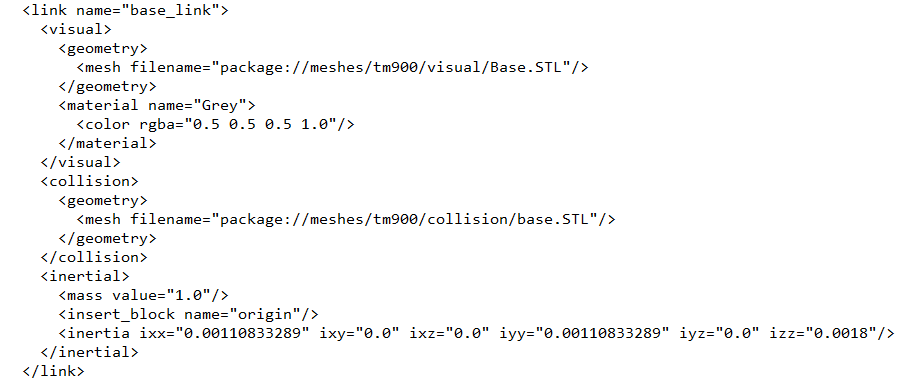
\includegraphics[width=0.5\textwidth]{images/URDF_Importer_5.png}
        \caption{URDF Importer Tutorial}
        \label{fig:URDF_Importer_5}
    \end{figure}
    \item Tasto destro sul file URDF e cliccare su "Import Robot from selected URDF file"
    \begin{figure}[H]
        \centering
        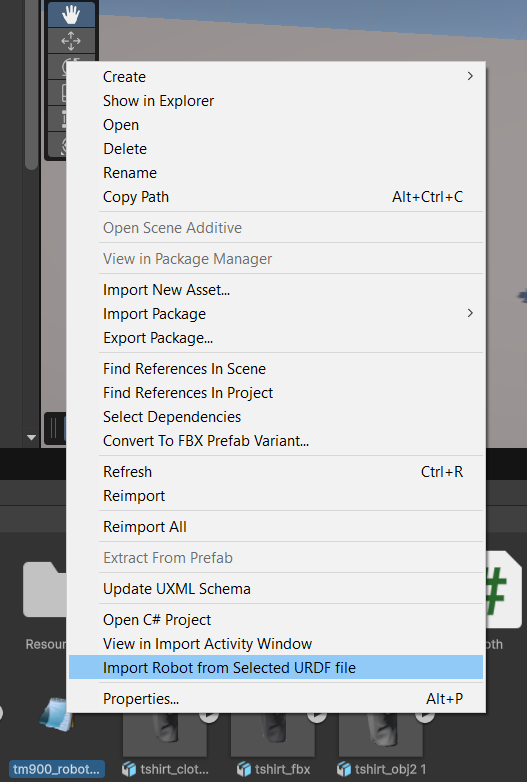
\includegraphics[width=0.35\textwidth]{images/URDF_Importer_6.png}
        \caption{URDF Importer Tutorial}
        \label{fig:URDF_Importer_6}
    \end{figure}
\end{itemize}

A questo punto, se è stato utilizzato il file urdf del TM5-900 corretto, sarà possibile visualizzare il robot come mostrato in figura \ref{fig:URDF_Importer_7}.
\begin{figure}[H]
    \centering
    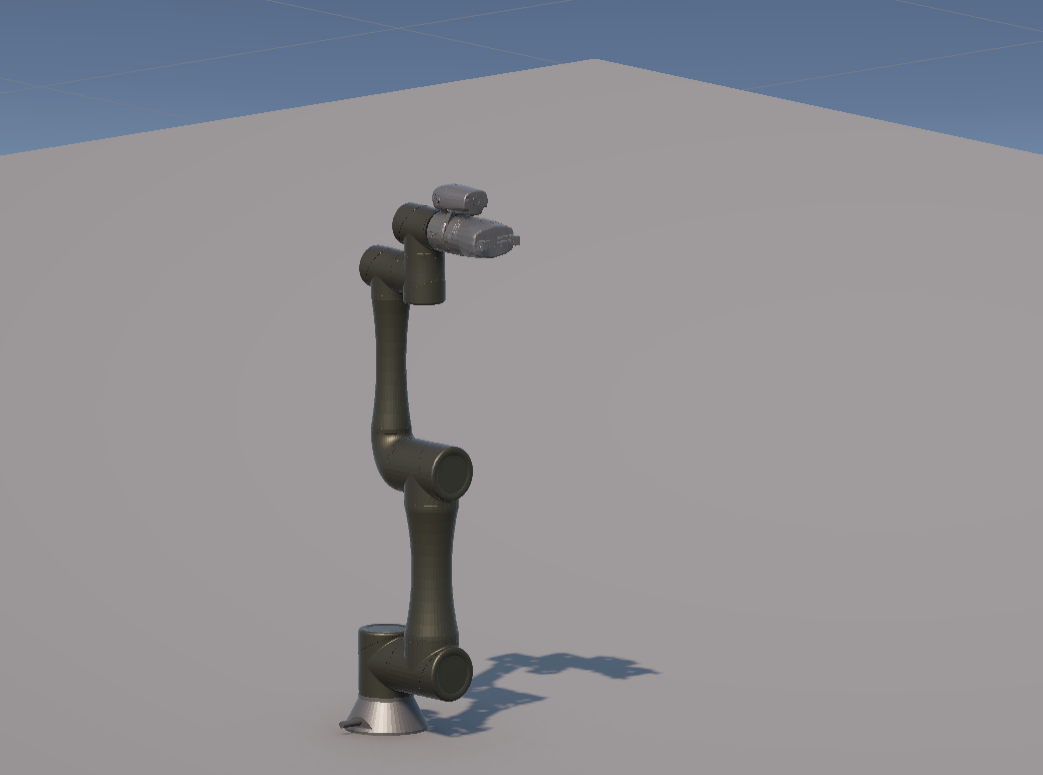
\includegraphics[width=0.35\textwidth]{images/URDF_Importer_7.png}
    \caption{URDF Importer Tutorial}
    \label{fig:URDF_Importer_7}     
\end{figure}

\section{Configurazione del Moveit Setup Assistant}
\label{sec:moveit_setup_assistant}
Di seguito sono riportati i passaggi svolti per la configurazione del package moveit\_config\_tm5\_900 utilizzando il MoveIt Setup Assistant \cite{Moveit_tutorial}: 
\begin{enumerate}
    \item Lanciamo il MoveIt Setup Assistant con il comando \begin{verbatim}
        roslaunch moveit_setup_assistant setup_assistant.launch
    \end{verbatim}
    \item Clicchiamo su "Create New MoveIt Configuration Package" e selezioniamo il file URDF del robot
    \item Nella sezione "Self Collision" è possibile generare automaticamente il controllo delle auto-collisioni del robot, selezionando "Generate Collision Matrix".
    \item Tramite "Virtual Joint" è possibile definire il giunto virtuale del robot, che rappresenta la connessione tra il robot e il mondo esterno. In questo caso, abbiamo selezionato "fixed" come tipo di giunto.
    \item Nella sezione "Planning Groups" aggiungere il gruppo "Manipulator" che comprende tutti i giunti a partire da "shoulder\_1\_ joint" fino a "wrist\_3\_joint". Se nel URDF è presente la pinza è possibile aggiungere anche il gruppo "Gripper".
    \item Successivamente tramite "Robot Poses" sono state definite due pose, una di riposo(Home) e una di lavoro(Work). In caso di aggiunta della pinza si possono definire due pose della pinza in modo che il robot possa afferrare oggetti e manipolarli.
    \item Infine generiamo i controllori "Ros2 Controllers" e "Ros2 MoveIt Controllers" per la comunicazione tra il robot e MoveIt. Per il nostro progetto abbiamo selezionato rispettivamente il controller "JointTrajectoryController" e "FollowJointTrajectory" per il gruppo "Manipulator".
    \item A questo punto rimane solo da generare il package tramite "Genera Package" nella sezione "Configurations Files".
\end{enumerate}

MoveIt ha svolto un ruolo centrale nell’interazione tra ROS 2 e Unity e ci ha permesso di simulare la movimentazione del robot solo tramite due codici, uno in C\# per Unity e uno in Python per ROS2, che verranno poi approfonditi nella sezione \ref{cap:Conclusioni}. Le traiettorie generate da MoveIt sono state pubblicate sul topic $/manipulator_controller/joint_trajectory$, successivamente sottoscritto in Unity tramite il pacchetto ROS-TCP Connector. Questo ha permesso una rappresentazione visiva coerente tra la pianificazione in ROS 2 e l’esecuzione nella simulazione 3D.

Inoltre è stato possibile utilizzare il package generato per avviare RViz, un potente strumento di visualizzazione per ROS, che consente di monitorare e analizzare i movimenti del robot in tempo reale. RViz è stato utilizzato per verificare la correttezza della pianificazione delle traiettorie e per eseguire test preliminari prima di passare alla simulazione in Unity.

Tramite il comando:
\begin{verbatim}
    ros2 launch moveit_config_tm5_900 demo.launch.py
\end{verbatim}

è possibile avviare il package generato e visualizzare il robot in RViz, in quanto l'URDF del robot è già presente nel package.

\begin{figure}[H]
    \centering
    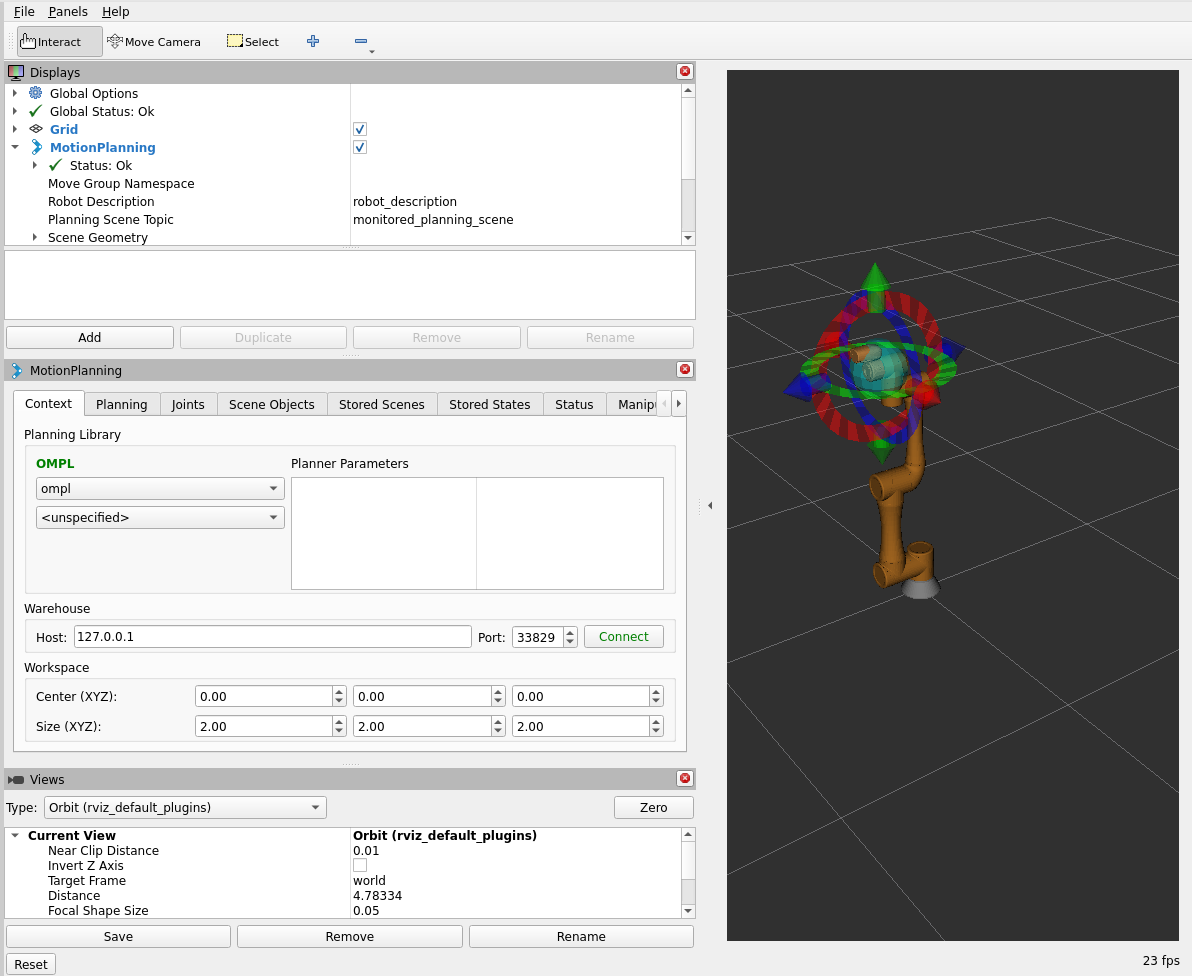
\includegraphics[width=0.9\textwidth]{images/rviz_1.PNG}
    \caption{Schermata iniziale RViz}
    \label{fig:rviz_1}
\end{figure}

Dalla figura \ref{fig:rviz_1} è possibile vedere la schermata iniziale una volta lanciato il comando sopra indicato.
A questo punto, nella sezione "Planning", indicando il gruppo di giunti, una posizione iniziale e finale del robot, come mostrato in figura \ref{fig:rviz_2}, RViz salverà le posizioni dei giunti di entrambe le pose. Successivamente, cliccando su "Plan \& Execute" il robot si muoverà nella posizione finale indicata, simulanod la traiettoria.

\begin{figure}[H]
    \centering
    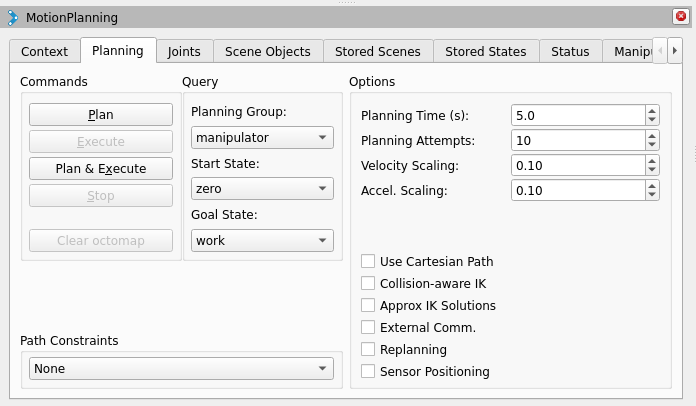
\includegraphics[width=0.7\textwidth]{images/rviz_2.PNG}
    \caption{Configurazione della pianificazione ed esecuzione della traiettoria in RViz}
    \label{fig:rviz_2}
\end{figure}

Non solo, tramite RViz è inoltre possibile creare nuove pose come mostrato in figura \ref{fig:rviz_3}, e testare le traiettorie in breve tempo.

\begin{figure}[H]
    \centering
    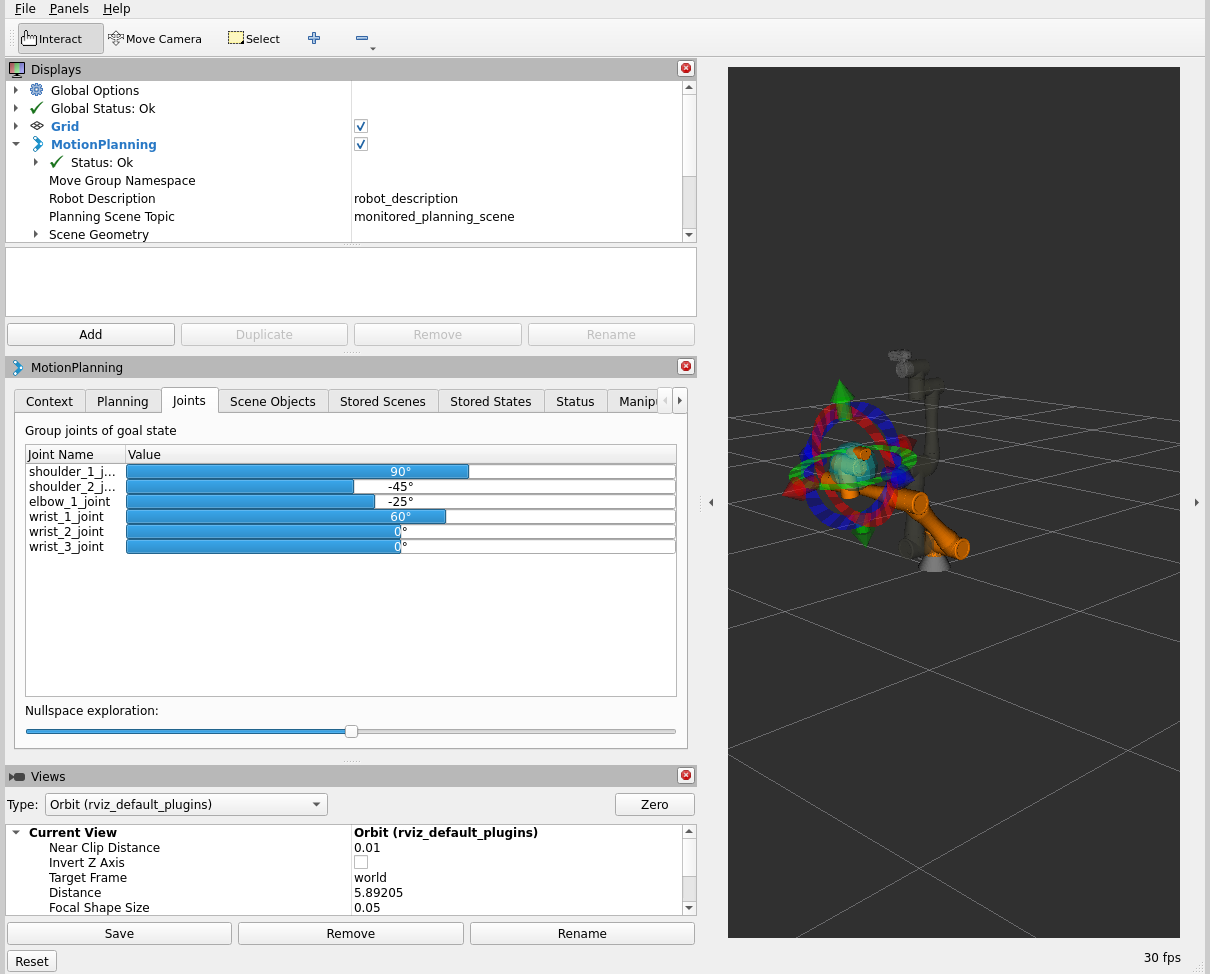
\includegraphics[width=0.7\textwidth]{images/rviz_3.PNG}
    \caption{Configurazione della posizione dei giunti in RViz}
    \label{fig:rviz_3}
\end{figure}

Nel mentre, è risultato molto utile controllare il terminale durante queste operazioni perché Moveit riportava eventuali errori o problemi di collisione tra il robot e l'ambiente circostante. Questo ha permesso di ottimizzare le traiettorie e garantire un movimento fluido e sicuro del robot.

\section{Importazione TM5-900 in Gazebo}
\label{sec:Importazione_TM5-900_Gazebo}

\subsubsection{URDF importer In Gazebo}
Il file URDF (\textit{Unified Robot Description Format}) è un file XML usato per rappresentare la struttura fisica, cinematica e dinamica di un robot. Questa descrizione è fondamentale per simulazioni, visualizzazioni 3D e per l'interazione con i sistemi ROS.
.

\subsubsection*{Struttura dell' URDF}

Tutti gli elementi sono racchiusi nel tag \texttt{<robot>}:

\begin{lstlisting}[language=xml]
<robot name="tm900">
    ...
</robot>
\end{lstlisting}

\subsubsection*{Descrizione dei Link}

Ogni \texttt{link} rappresenta una parte rigida del robot. Ogni link include:

\begin{itemize}
    \item \texttt{<visual>} – descrizione visiva (mesh o primitiva)
    \item \texttt{<collision>} – forma per la collisione
    \item \texttt{<inertial>} – massa, centro di massa e inerzia
\end{itemize}

Esempio per il link \texttt{shoulder\_1\_link}:

\begin{lstlisting}[language=xml]
<link name="shoulder_1_link">
  <visual>
    <geometry>
      <mesh filename="package://tm900/meshes/shoulder_1.stl"/>
    </geometry>
    <material name="grey"/>
  </visual>
  <collision>
    <geometry>
      <mesh filename="package://tm900/meshes/shoulder_1.stl"/>
    </geometry>
  </collision>
  <inertial>
    <mass value="2.5"/>
    <origin xyz="0 0 0" rpy="0 0 0"/>
    <inertia
      ixx="0.03" ixy="0.0" ixz="0.0"
      iyy="0.03" iyz="0.0"
      izz="0.03"/>
  </inertial>
</link>
\end{lstlisting}

\subsubsection*{Descrizione dei Joint}

I \texttt{joint} collegano due link tra loro e ne definiscono il tipo di movimento relativo. Ogni joint contiene:

\begin{itemize}
    \item \texttt{name}, \texttt{type} (revolute, fixed, prismatic, ecc.)
    \item \texttt{<parent>} e \texttt{<child>}
    \item \texttt{<origin>} – posizione e orientamento del giunto
    \item \texttt{<axis>} – direzione dell’asse di rotazione
    \item \texttt{<limit>} – limiti meccanici (per giunti mobili)
\end{itemize}

Esempio:

\begin{lstlisting}[language=xml]
<joint name="shoulder_1_joint" type="revolute">
  <parent link="base_link"/>
  <child link="shoulder_1_link"/>
  <origin xyz="0 0 0.1" rpy="0 0 0"/>
  <axis xyz="0 0 1"/>
  <limit lower="-3.14" upper="3.14" effort="20" velocity="1.0"/>
</joint>
\end{lstlisting}

\subsubsection*{Proprietà Fisiche}

Le proprietà fisiche sono definite nei blocchi \texttt{<inertial>} e \texttt{<collision>} di ogni link. Queste includono:

\begin{itemize}
    \item \textbf{Massa} – specificata in kg
    \item \textbf{Momento d’inerzia} – matrice 3x3, usata per simulazioni dinamiche
    \item \textbf{Collisioni} – geometrie per il rilevamento delle collisioni
    \item \textbf{Materiali} – colore e aspetto visivo
\end{itemize}

\section*{Trasmissioni e Controllo}

Il controllo avviene tramite plugin ROS. Ogni giunto attuato ha una trasmissione:

\begin{lstlisting}[language=xml]
<transmission name="elbow_trans">
  <type>transmission_interface/SimpleTransmission</type>
  <joint name="elbow_joint">
    <hardwareInterface>PositionJointInterface</hardwareInterface>
  </joint>
  <actuator name="elbow_motor">
    <hardwareInterface>PositionJointInterface</hardwareInterface>
    <mechanicalReduction>1</mechanicalReduction>
  </actuator>
</transmission>
\end{lstlisting}

\subsubsection*{Simulazione in Gazebo}

Per la simulazione in Gazebo si definisce il plugin:

\begin{lstlisting}[language=xml]
<gazebo>
  <plugin name="gazebo_ros_control" filename="libgazebo_ros_control.so"/>
</gazebo>
\end{lstlisting}

Per ogni link si può abilitare la self-collision:

\begin{lstlisting}[language=xml]
<gazebo reference="wrist_link">
  <selfCollide>true</selfCollide>
</gazebo>
\end{lstlisting}

\subsubsection*{Problema con la visualizzazione delle Mesh}

Durante il processo di sviluppo del modello URDF del robot TM900, è stato riscontrato un problema relativo alla visualizzazione delle mesh in Gazebo. Sebbene l'oggetto venisse correttamente creato nel mondo Gazebo, non veniva visualizzato graficamente. Dopo una serie di verifiche, si è scoperto che il problema derivava dal fatto che le mesh non erano correttamente localizzate nel path di installazione.

La soluzione adottata è stata quella di spostare i file delle mesh nel path di install del pacchetto. In particolare, sono stati inseriti all'interno della cartella:

\begin{quote}
\texttt{package://tm900/meshes/}
\end{quote}

Questo ha permesso a Gazebo di localizzare correttamente i file e di visualizzare il robot senza ulteriori problemi.


\section{Camera}

\subsection{Introduzione}
La camera Intel RealSense D435i è un dispositivo avanzato per la rilevazione della profondità, dotato di sensore IMU integrato che consente l'acquisizione simultanea di dati visivi e inerziali. Grazie alla combinazione di una coppia di sensori stereo e di una fotocamera RGB, la D435i è ampiamente utilizzata in applicazioni di robotica, visione artificiale, mappatura 3D e realtà aumentata.

\subsection{Configurazione Iniziale}
\subsubsection{Setup della Camera Virtuale}
\begin{itemize}
\item Eliminare l'oggetto \texttt{mainCamera} predefinito
\item Creare un nuovo oggetto Camera dal menu GameObject
\item Rinominarlo \texttt{realSenseCamera}
\item Impostare il Field Of View a 87°
\end{itemize}

\begin{figure}[H]
    \centering
    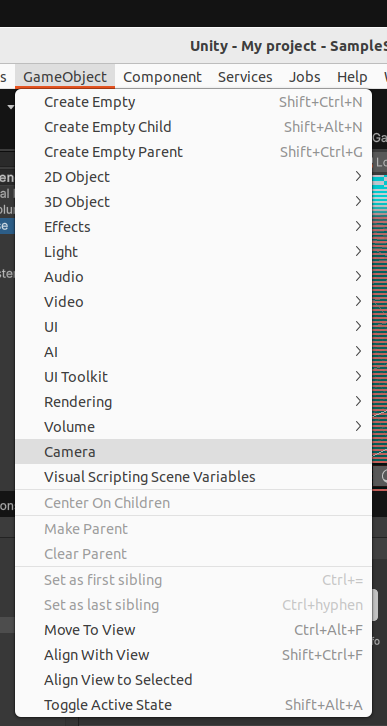
\includegraphics[width=0.8\textwidth]{images/Immagine1.png}
    \caption{Creazione dell'oggetto camera in Unity}
    \label{fig:create_camera}
\end{figure}

\begin{figure}[H]
    \centering
    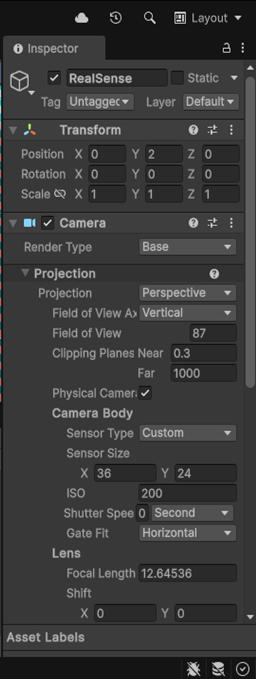
\includegraphics[width=0.8\textwidth]{images/Immagine2.png}
    \caption{Impostazione del Field Of View}
    \label{fig:fov_setting}
\end{figure}

\subsection{Preparazione Scena}
\begin{itemize}
\item Aggiungere una sfera come oggetto di test
\item Assegnare materiali e colori
\item Configurare l'illuminazione base
\end{itemize}

\begin{figure}[H]
    \centering
    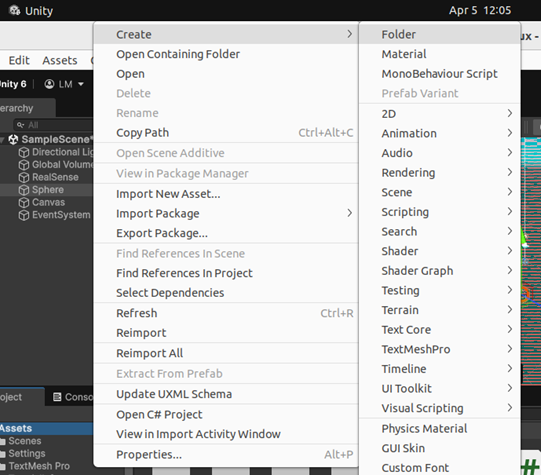
\includegraphics[width=0.8\textwidth]{Immagine3.png}
    \caption{Inserimento del materiale e colore alla sfera}
    \label{fig:sphere_material}
\end{figure}

\section{Implementazione Base}
\begin{lstlisting}[caption=Script base di acquisizione immagini, label=lst:base, lineskip=0.3em]
using UnityEngine;
using System.IO;

[RequireComponent(typeof(Camera))]
public class RealSenseSimulator : MonoBehaviour
{
    public Camera realSenseCamera;
    private RenderTexture renderTexture;
    private Texture2D colorTexture2D;
    private Texture2D depthTexture2D;

    void Start()
    {
        renderTexture = new RenderTexture(1280, 720, 24, 
            RenderTextureFormat.ARGB32);
        realSenseCamera.targetTexture = renderTexture;
        realSenseCamera.depthTextureMode = DepthTextureMode.Depth;
        
        colorTexture2D = new Texture2D(1280, 720, 
            TextureFormat.RGB24, false);
        depthTexture2D = new Texture2D(1280, 720, 
            TextureFormat.RGB24, false);
    }

    void Update()
    {
        RenderTexture.active = renderTexture;
        colorTexture2D.ReadPixels(new Rect(0, 0, 1280, 720), 0, 0);
        colorTexture2D.Apply();
        
        SaveRGBValuesToFile();
        SaveRGBImage();
        StartCoroutine(CaptureDepth());
    }

    private void SaveRGBValuesToFile()
    {
        string filePath = "Assets/rgb_values.csv";
        using (StreamWriter writer = new StreamWriter(filePath, false))
        {
            writer.WriteLine("X,Y,R,G,B");
            for (int y = 0; y < colorTexture2D.height; y++)
            {
                for (int x = 0; x < colorTexture2D.width; x++)
                {
                    Color pixelColor = colorTexture2D.GetPixel(x, y);
                    writer.WriteLine($"{x},{y},{
                        pixelColor.r * 255},{
                        pixelColor.g * 255},{
                        pixelColor.b * 255}");
                }
            }
        }
        Debug.Log("RGB values saved to " + filePath);
    }

    private void SaveRGBImage()
    {
        byte[] rgbData = colorTexture2D.EncodeToPNG();
        File.WriteAllBytes(
            Application.dataPath + "/simulated_rgb_image.png", 
            rgbData);
    }

    private IEnumerator CaptureDepth()
    {
        yield return new WaitForEndOfFrame();
        
        RenderTexture depthRT = RenderTexture.GetTemporary(
            1280, 720, 24, RenderTextureFormat.Depth);
        Graphics.Blit(null, depthRT, 
            new Material(Shader.Find(
                "Hidden/Internal-DepthNormalsTexture")));
        
        RenderTexture.active = depthRT;
        Texture2D tempDepth = new Texture2D(1280, 720, 
            TextureFormat.RFloat, false);
        tempDepth.ReadPixels(new Rect(0, 0, 1280, 720), 0, 0);
        tempDepth.Apply();

        for (int y = 0; y < depthTexture2D.height; y++)
        {
            for (int x = 0; x < depthTexture2D.width; x++)
            {
                float depthValue = tempDepth.GetPixel(x, y).r;
                Color gray = new Color(depthValue, 
                    depthValue, depthValue);
                depthTexture2D.SetPixel(x, y, gray);
            }
        }
        depthTexture2D.Apply();

        byte[] depthData = depthTexture2D.EncodeToPNG();
        File.WriteAllBytes(
            Application.dataPath + "/simulated_depth_image.png", 
            depthData);

        RenderTexture.ReleaseTemporary(depthRT);
        Destroy(tempDepth);
        Debug.Log("Depth image saved.");
    }
}
\end{lstlisting}

\begin{figure}[H]
    \centering
    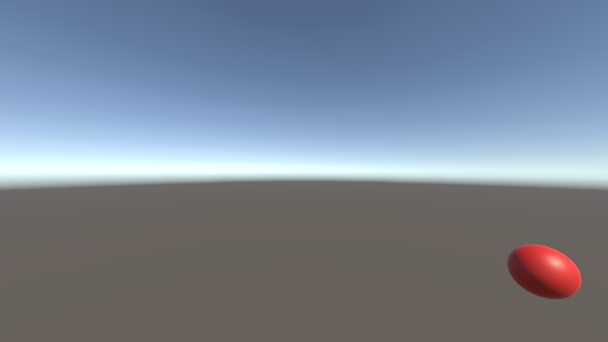
\includegraphics[width=0.8\textwidth]{Immagine4.png}
    \caption{Immagine creata in formato PNG}
    \label{fig:output_image}
\end{figure}

\subsection{L'algoritmo base}
\onehalfspacing
Attraverso l'utilizzo di una camera virtuale e di una RenderTexture, il sistema acquisisce i dati visivi della scena e li converte in texture gestibili tramite Texture2D.
 Ogni n frame, i dati RGB vengono esportati in formato .png e salvati anche in un file .csv, consentendo un'analisi dettagliata dei singoli pixel. Contestualmente, viene generata una mappa di profondità simulata mediante una funzione sinusoidale che varia nel tempo, permettendo una rappresentazione dinamica della distanza. Una sezione specifica dello script è inoltre dedicata alla simulazione di variazioni visive e di profondità localizzate, al fine di testare la sensibilità del sistema nel rilevare modifiche. L’architettura del codice è orientata all’efficienza e alla modularità, risultando adatta a scenari di test e sviluppo per sistemi di visione artificiale basati su dati RGB-D.
La simulazione della profondità è stata realizzata tramite una funzione periodica per garantire un controllo preciso e dinamico dei valori di profondità, senza la necessità di un sensore fisico. Questo approccio consente di testare il comportamento del sistema in modo riproducibile. Inoltre, permette di verificare l’integrazione e la sincronizzazione tra il flusso visivo e quello di profondità in un contesto completamente simulato.
 Il metodo GenerateDepthData() simula una mappa di profondità generando valori di intensità in scala di grigi per ogni pixel, utilizzando una funzione sinusoidale che varia nel tempo. Questo crea un effetto ondulato e dinamico, utile per testare il comportamento di sistemi basati su dati di profondità senza l’uso di un sensore fisico.

\section{Integrazione ROS2 nell'algoritmo base}
\subsection{requisiti di Sistema}
\begin{itemize}
\item Pubblicazione su due topic separati (RGB e Depth)
\item Frequenza: 10Hz (0.1 secondi)
\item Utilizzo del pacchetto Unity-Robotics-ROSTCPConnector
\item Formato messaggi ROS standard
\end{itemize}
\vspace{-1em} % rimuove spazio tra caption e codice
\begin{lstlisting}[caption=Integrazione dello script di Ros2, label=lst:base, lineskip=0.3em]
using UnityEngine;
using System.IO;
using System.Collections;
using Unity.Robotics.ROSTCPConnector;
using RosMessageTypes.Sensor;

[RequireComponent(typeof(Camera))]
public class RealSenseSimulator : MonoBehaviour
{
    public Camera realSenseCamera;
    private RenderTexture renderTexture;
    private Texture2D colorTexture2D;
    private Texture2D depthTexture2D;
    
    public float publishInterval = 0.1f;
    private float nextPublishTime = 0f;
    public string colorTopic = "/camera/color/image_raw";
    public string depthTopic = "/camera/depth/image_raw";
    private ROSConnection ros;

    void Start()
    {
        ros = ROSConnection.instance;
        ros.RegisterPublisher<ImageMsg>(colorTopic);
        ros.RegisterPublisher<ImageMsg>(depthTopic);

        renderTexture = new RenderTexture(1280, 720, 24, 
            RenderTextureFormat.ARGB32);
        realSenseCamera.targetTexture = renderTexture;
        realSenseCamera.depthTextureMode = DepthTextureMode.Depth;
        
        colorTexture2D = new Texture2D(1280, 720, 
            TextureFormat.RGB24, false);
        depthTexture2D = new Texture2D(1280, 720, 
            TextureFormat.R8, false);
    }

    void Update()
    {
        RenderTexture.active = renderTexture;
        colorTexture2D.ReadPixels(new Rect(0, 0, 1280, 720), 0, 0);
        colorTexture2D.Apply();
        
        StartCoroutine(CaptureDepth());

        if (Time.time >= nextPublishTime)
        {
            PublishRGBD();
            nextPublishTime = Time.time + publishInterval;
        }
    }

    private void PublishRGBD()
    {
        ImageMsg colorMsg = new ImageMsg
        {
            header = new StdMsgs.HeaderMsg { 
                frame_id = "camera_color_frame" },
            height = (uint)colorTexture2D.height,
            width = (uint)colorTexture2D.width,
            encoding = "rgb8",
            step = (uint)(colorTexture2D.width * 3),
            data = colorTexture2D.GetRawTextureData()
        };

        ImageMsg depthMsg = new ImageMsg
        {
            header = new StdMsgs.HeaderMsg { 
                frame_id = "camera_depth_frame" },
            height = (uint)depthTexture2D.height,
            width = (uint)depthTexture2D.width,
            encoding = "mono8",
            step = (uint)(depthTexture2D.width * 1),
            data = depthTexture2D.GetRawTextureData()
        };

        ros.Publish(colorTopic, colorMsg);
        ros.Publish(depthTopic, depthMsg);
    }

    private IEnumerator CaptureDepth()
    {
        yield return new WaitForEndOfFrame();
        
        RenderTexture depthRT = RenderTexture.GetTemporary(
            1280, 720, 0, RenderTextureFormat.ARGBFloat);
        Material depthMat = new Material(
            Shader.Find("Hidden/Internal-DepthNormalsTexture"));
        
        Graphics.Blit(null, depthRT, depthMat);
        RenderTexture.active = depthRT;
        
        Texture2D tempDepth = new Texture2D(1280, 720, 
            TextureFormat.RGBAFloat, false);
        tempDepth.ReadPixels(new Rect(0, 0, 1280, 720), 0, 0);
        tempDepth.Apply();

        for (int y = 0; y < depthTexture2D.height; y++)
        {
            for (int x = 0; x < depthTexture2D.width; x++)
            {
                float d = tempDepth.GetPixel(x, y).a;
                depthTexture2D.SetPixel(x, y, new Color(d, 0f, 0f));
            }
        }
        depthTexture2D.Apply();

        RenderTexture.ReleaseTemporary(depthRT);
        Destroy(tempDepth);
    }
}
\end{lstlisting}
\subsection{Descrizione dello script \texttt{RealSenseSimulator.cs}}

Lo script \texttt{RealSenseSimulator.cs}, scritto in C\#, è progettato per simulare il comportamento di una telecamera RealSense all'interno di Unity, con la capacità di acquisire immagini a colori e mappe di profondità, e di pubblicarle tramite ROS~2 utilizzando il pacchetto \texttt{Unity.Robotics.ROSTCPConnector}.

\paragraph{Componenti principali}
Lo script è associato ad un oggetto Unity contenente una \texttt{Camera}, il cui output visivo viene catturato e trasformato in messaggi \texttt{sensor\_msgs/Image} compatibili con ROS~2. Il comportamento dello script è articolato nei seguenti punti principali:

\begin{itemize}
  \item \textbf{Inizializzazione:} Nella funzione \texttt{Start()}, viene creato un \texttt{RenderTexture} con risoluzione 1280$\times$720 e formato ARGB32. Questo buffer viene assegnato come output della telecamera per la cattura dei frame a colori. Inoltre, viene abilitato il \texttt{DepthTextureMode.Depth} per permettere la generazione automatica della mappa di profondità. Vengono quindi inizializzate due texture 2D: una per il colore (\texttt{RGB24}) e una per la profondità (\texttt{R8}).
  
  \item \textbf{Integrazione con ROS 2:} Viene ottenuta l’istanza di \texttt{ROSConnection}, alla quale sono registrati due publisher per i topic \texttt{/camera/color/image\_raw} e \texttt{/camera/depth/image\_raw}, entrambi configurati per inviare messaggi di tipo \texttt{ImageMsg}.
\end{itemize}

\paragraph{Funzionamento in tempo reale}
All'interno della funzione \texttt{Update()}, chiamata ad ogni frame da Unity, avvengono le seguenti operazioni:
\begin{enumerate}
  \item Il contenuto del \texttt{RenderTexture} attivo viene letto nella \texttt{colorTexture2D} mediante \texttt{ReadPixels}, catturando il frame RGB.
  \item Viene avviata la coroutine \texttt{CaptureDepth()}, che esegue in modo asincrono la cattura della profondità.
  \item Se è trascorso l'intervallo di pubblicazione definito (\texttt{publishInterval}), vengono pubblicati i dati RGB e di profondità tramite la funzione \texttt{PublishRGBD()}.
\end{enumerate}

\paragraph{Pubblicazione dei dati}
Il metodo \texttt{PublishRGBD()} crea due oggetti \texttt{ImageMsg}, uno per l’immagine RGB e uno per la profondità, impostando opportunamente il frame di riferimento, risoluzione, encoding e passo (\texttt{step}). I dati grezzi delle texture vengono letti tramite \texttt{GetRawTextureData()} e assegnati ai rispettivi messaggi. Infine, i messaggi vengono pubblicati sui topic ROS specificati.

\paragraph{Cattura della profondità}
La funzione \texttt{CaptureDepth()} è una coroutine che utilizza un \texttt{RenderTexture} temporaneo in formato \texttt{ARGBFloat} per acquisire la mappa di profondità. Questo viene ottenuto applicando un materiale con shader interno \texttt{Hidden/Internal-DepthNormalsTexture}, che consente di generare una texture contenente informazioni di profondità.

La profondità viene letta in una texture temporanea in formato \texttt{RGBAFloat}. Per ciascun pixel, il canale alfa rappresenta la profondità normalizzata, che viene poi convertita in un'immagine a canale singolo scrivendo il valore nel canale rosso della \texttt{depthTexture2D}. La texture risultante viene infine utilizzata per la pubblicazione ROS.

\paragraph{Nota sull'efficienza}
Va notato che la conversione della profondità pixel-per-pixel e la distruzione dinamica delle texture temporanee possono introdurre un overhead computazionale significativo, specialmente in scenari ad alta frequenza di pubblicazione. In contesti più esigenti, si potrebbe considerare l'ottimizzazione attraverso l'elaborazione GPU-side o tecniche di bufferizzazione.

\paragraph{Conclusione}
In sintesi, lo script \texttt{RealSenseSimulator} fornisce un'integrazione completa tra Unity e ROS~2 per la simulazione di sensori RGB-D. Esso consente lo sviluppo e la validazione di sistemi robotici in ambienti virtuali realistici, mantenendo una struttura modulare e compatibile con l'infrastruttura ROS.

\subsection{Subscriber ROS2}
\begin{lstlisting}[language=Python, caption=Subscriber RGB-D ROS2 con salvataggio video, label=lst:rgbd_subscriber]
#!/usr/bin/env python3
import rclpy
from rclpy.node import Node
from sensor_msgs.msg import Image
from cv_bridge import CvBridge, CvBridgeError
import cv2

class RGBDSubscriber(Node):
    def __init__(self):
        super().__init__('rgbd_subscriber')
        self.bridge = CvBridge()
        # File video di output
        fourcc = cv2.VideoWriter_fourcc(*'XVID')
        width, height = 1280, 720
        fps = 10.0  # 10 fps in linea con Unity
        self.rgb_writer = cv2.VideoWriter('output_rgb.avi', fourcc, fps, (width, height))
        self.depth_writer = cv2.VideoWriter('output_depth.avi', fourcc, fps, (width, height), isColor=False)

        if not self.rgb_writer.isOpened():
            self.get_logger().error('Impossibile aprire output_rgb.avi') 
        if not self.depth_writer.isOpened():
            self.get_logger().error('Impossibile aprire output_depth.avi') 

        # Subscriber per colore e profondità
        self.create_subscription(Image, '/camera/color/image_raw', self.color_callback, 10)
        self.create_subscription(Image, '/camera/depth/image_raw', self.depth_callback, 10)

        self.shutdown_timer = self.create_timer(
            60.0,                 # periodo in secondi
            self.shutdown_callback  # callback di chiusura
        )

    def color_callback(self, msg: Image):
        try:
            # Converte in BGR8 (OpenCV usa BGR)
            cv_image = self.bridge.imgmsg_to_cv2(msg, desired_encoding='rgb8')
            cv_image = cv2.cvtColor(cv_image, cv2.COLOR_RGB2BGR)

            # Ruota di 180 gradi
            rotated = cv2.rotate(cv_image, cv2.ROTATE_180)
            cv2.imshow('Color View', rotated)

            # Scrive sul video
            self.rgb_writer.write(rotated)

        except CvBridgeError as e:
            self.get_logger().error(f'CVBridge Error: {e}')
        
        cv2.waitKey(1)

    def depth_callback(self, msg: Image):
        try:
            # Converte direttamente in gray-scale 8-bit
            gray = self.bridge.imgmsg_to_cv2(msg, desired_encoding='mono8')

            # Visualizza la depth
            cv2.imshow('Depth View', gray)

            # Scrive nel video
            self.depth_writer.write(gray)

        except CvBridgeError as e:
            self.get_logger().error(f'CVBridge Error (Depth): {e}')

        cv2.waitKey(1)

    def destroy_node(self):
        super().destroy_node()

    def shutdown_callback(self):
        self.get_logger().info('Timeout raggiunto: fermo acquisizione e chiudo finestre.')
        self.rgb_writer.release()
        self.depth_writer.release()
        cv2.destroyAllWindows()
        self.shutdown_timer.cancel()
        self.destroy_node()
        rclpy.shutdown()

def main(args=None):
    rclpy.init(args=args)
    node = RGBDSubscriber()
    rclpy.spin(node)

if __name__ == '__main__':
    main()
\end{lstlisting}
\subsection{Descrizione del nodo \texttt{RGBDSubscriber}}

Il nodo \texttt{RGBDSubscriber} in ambiente ROS~2 ha il compito di acquisire, visualizzare e registrare in formato video i flussi RGB e di profondità (Depth) provenienti da una telecamera simulata. I dati sono pubblicati su due topic ROS distinti, rispettivamente per il colore e la profondità. Il nodo è implementato in Python e fa uso delle librerie \texttt{rclpy} per la comunicazione con ROS~2, \texttt{sensor\_msgs.msg.Image} per la gestione dei messaggi di immagine, \texttt{cv\_bridge} per la conversione tra formati ROS e strutture compatibili con OpenCV, e \texttt{opencv-python} per l’elaborazione e visualizzazione delle immagini.

\paragraph{Inizializzazione}
Nel costruttore della classe \texttt{RGBDSubscriber}, viene inizializzato un oggetto \texttt{CvBridge} per la conversione tra messaggi ROS e immagini OpenCV. Successivamente, vengono creati due oggetti \texttt{cv2.VideoWriter} per la registrazione dei video RGB e di profondità, utilizzando il codec \texttt{XVID}, una risoluzione di 1280$\times$720 pixel e una frequenza di 10~fps, in linea con la frequenza di pubblicazione del simulatore Unity.

Il nodo si sottoscrive ai seguenti topic:
\begin{itemize}
  \item \texttt{/camera/color/image\_raw} per le immagini RGB;
  \item \texttt{/camera/depth/image\_raw} per le immagini di profondità.
\end{itemize}

Viene inoltre impostato un \textit{timer} di spegnimento automatico a 60 secondi, che richiama una procedura di chiusura controllata.

\paragraph{Gestione del flusso RGB}
Il metodo \texttt{color\_callback} viene eseguito ad ogni ricezione di un messaggio RGB. L’immagine viene convertita nel formato \texttt{BGR8}, ruotata di 180° per correggere l’orientamento, visualizzata in una finestra OpenCV denominata \texttt{"Color View"} e registrata nel file \texttt{output\_rgb.avi}. La chiamata a \texttt{cv2.waitKey(1)} permette l’aggiornamento dell’interfaccia grafica di OpenCV.

\paragraph{Gestione del flusso di profondità}
In modo analogo, il metodo \texttt{depth\_callback} converte il messaggio ROS nel formato \texttt{mono8} (scala di grigi a 8 bit), visualizza il risultato nella finestra \texttt{"Depth View"} e lo registra nel file \texttt{output\_depth.avi}. Anche in questo caso, \texttt{cv2.waitKey(1)} consente la corretta gestione delle finestre OpenCV.

\paragraph{Procedura di arresto}
Trascorsi 60 secondi, il metodo \texttt{shutdown\_callback} viene eseguito automaticamente. Esso:
\begin{itemize}
  \item stampa un messaggio di log;
  \item rilascia i \texttt{VideoWriter} per completare i file video;
  \item chiude tutte le finestre di OpenCV;
  \item cancella il timer ed esegue la distruzione del nodo;
  \item richiama \texttt{rclpy.shutdown()} per arrestare ROS~2.
\end{itemize}

\paragraph{Funzione \texttt{main}}
La funzione \texttt{main()} inizializza l'ambiente ROS~2, crea un’istanza del nodo e mantiene attiva l’elaborazione degli eventi attraverso \texttt{rclpy.spin()}, fino alla terminazione del nodo stesso.

\subsection{Output Base}
\begin{itemize}
\item File RGB in formato PNG e CSV
\item Mappa di profondità in scala di grigi
\item Salvataggio automatico nella cartella Assets
\end{itemize}

\subsection{Output ROS2}
\begin{itemize}
\item Flusso video RGB funzionante
\item Problemi con dati di profondità:
\begin{itemize}
    \item Immagini piatte
    \item Mancanza di variazioni
    \item Possibili cause:
    \begin{itemize}
        \item Impostazioni camera
        \item Shader di profondità
        \item Conversione formato
    \end{itemize}
\end{itemize}
\end{itemize}

\section{Conclusioni}
\subsection{Risultati dell'implememntazione della Camera}
\begin{figure}[H]
    \centering
    \begin{subfigure}{0.45\textwidth}
        \centering
        \includegraphics[width=\textwidth]{images/rgb_results.png}
        \caption{Risultato RGB}
    \end{subfigure}
    \begin{subfigure}{0.45\textwidth}
        \centering
        \includegraphics[width=\textwidth]{images/depth_results.png}
        \caption{Risultato profondità}
    \end{subfigure}
    \caption{Risultati dell'acquisizione}
    \label{fig:results}
\end{figure}
\subsection{Limitazioni}
\begin{itemize}
\item Profondità non completamente realistica
\item Dipendenza da shader Unity
\item Throughput non ottimizzato
\end{itemize}


\chapter{Analisi Preliminari e Problematiche Riscontrate}
\label{sec:Problemi}
\section{Problematiche sulle Compatibilità dei Software Utilizzati}
\label{sec:Problemi_Compatibilità}
Nel contesto del progetto, l’integrazione tra Unity e ROS2 rappresenta una sfida notevole dal punto di vista della compatibilità software. L’armonizzazione degli ambienti di simulazione grafica e del framework robotico comporta l’allineamento di versioni, librerie e tool, dove eventuali discrepanze possono causare malfunzionamenti, comportamenti inattesi e difficoltà nel mantenimento della comunicazione affidabile fra i sistemi. In generale, le principali problematiche riguardano:
\begin{itemize}
    \item \textbf{Dipendenze e Librerie}: Ogni ambiente software si basa su set specifici di dipendenze e librerie. Una discrepanza nelle versioni o nelle configurazioni può portare a malfunzionamenti, crash o comportamenti inattesi.

    \item \textbf{Protocollo di Comunicazione}: L’interfacciamento tramite strumenti come il ROS-TCP Connector \& Endpoint impone un rigoroso rispetto degli standard di serializzazione e deserializzazione dei messaggi. Differenze nelle versioni possono influenzare la compatibilità dei protocolli, rendendo critica la coerenza delle implementazioni.
    
    \item \textbf{Ambiente di Esecuzione e Simulazione}: La perfetta integrazione tra il motore fisico di Unity e il middleware ROS2 richiede una sincronizzazione accurata dei tempi di esecuzione, in modo da garantire una simulazione fluida e reattiva. Eventuali incompatibilità possono compromettere le performance e l’efficacia dei test simulativi.
\end{itemize}

Durante le fasi iniziali di sviluppo, il gruppo ha scelto di utilizzare ROS2 Jazzy, una distribuzione che, è supportata fino a maggio 2029, e rappresentava una versione più nuova e all’avanguardia. Tuttavia, in fase di integrazione con Unity sono emerse alcune criticità, in particolare durante i test si sono riscontrate carenze funzionali nelle librerie e nei tool di ROS2 Jazzy. Queste mancanze evidenziavano dei limiti, in particolare per quanto riguarda la robustezza delle comunicazioni e la gestione dei messaggi in ambienti complessi.
\newline
La migrazione verso ROS2 Humble è stata dettata dalla necessità di disporre di una versione più consolidata e con una maggiore compatibilità con gli strumenti attuali di Unity. ROS2 Humble, supportato fino a maggio 2027, ha offerto miglioramenti in termini di performance, stabilità e aggiornamenti, garantendo una maggiore robustezza nelle comunicazioni e nella gestione delle dipendenze. \cite{Supporto-versioni-ROS}
\newline
Chiaramente, con la scelta di passare a ROS2-Humble anche gli altri software utilizzati sono stati aggiornati, in particolare Gazebo è stato aggiornato alla versione Fortress, che ha mostrato una maggiore stabilità e compatibilità con ROS2 Humble. \cite{Gazebo-ROS2}
\newline
Con l’evolversi del progetto e l’avvicinarsi della scadenza del supporto per Humble, si dovrà valutare attentamente una futura migrazione verso ROS2 Jazzy. Passare a Jazzy in un secondo momento potrebbe permettere di sfruttare i miglioramenti continui offerti dalla nuova distribuzione, garantendo così una maggiore longevità e integrazione degli aggiornamenti nell’ecosistema software del progetto.
\section{Compatibilità dei File 3D con Unity e Gazebo}
\label{sec:Problemi_Compatibilità_3D}
Il formato \textbf{.obj} è stato testato con successo sia in Unity che in Gazebo, consentendo l'importazione corretta del modello della t-shirt in entrambi i software. Tuttavia, durante le simulazioni in Unity, l'applicazione del componente Cloth alla t-shirt ha evidenziato alcune difficoltà: il computer ha riscontrato problemi nel gestire correttamente i comandi impostati e, una volta avviata la simulazione, la t-shirt appariva deformata e non realistica, come è possibile vedere nella figura \ref{fig:cloth_error}.

\begin{figure}[H]
    \centering
    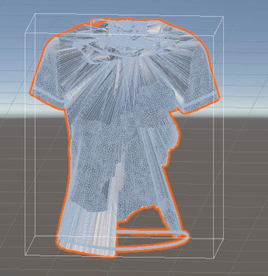
\includegraphics[width=0.4\textwidth]{images/cloth_error.PNG}
    \caption{Errore nell'applicazione del Cloth di Unity}
    \label{fig:cloth_error}
\end{figure}

Per risolvere questo problema, l'oggetto è stato importato nel software Blender, dove è stato utilizzato il modificatore Decimate per ridurre il numero di poligoni della mesh. Diminuendo il parametro "Ratio" a un valore che ha portato la mesh a circa 5000 poligoni, è stato possibile reimportare l'oggetto in Unity e applicare correttamente il componente Cloth, ottenendo una simulazione più realistica.

\begin{figure}[H]
    \centering
    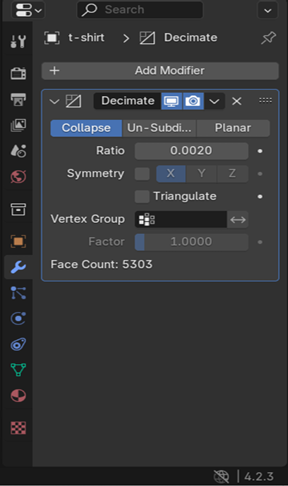
\includegraphics[width=0.3\textwidth]{images/blender_ratio.PNG}
    \caption{Modifica della Mesh nel software Blender}
    \label{fig:blender_ratio}
\end{figure}

Il formato \textbf{.fbx} non è supportato da Gazebo; tuttavia, è compatibile con Unity e può essere convertito in altri formati, come .obj o .dae (Collada), utilizzando Blender. Seguendo lo stesso procedimento adottato per il file .obj, quindi riducendo il numero di poligoni delle mesh tramite il modificatore Decimate in Blender, la simulazione in Unity è stata eseguita correttamente.

Il formato  \textbf{.dae} (Collada) è supportato da Gazebo e risulta essere ampiamente utilizzato in questo contesto. Importando i file .obj della t-shirt e della scarpa, nonché il file .fbx della t-shirt in Blender, è stato possibile esportarli nel formato .dae. Questa operazione ha permesso di caricare correttamente i vari modelli in Gazebo, facilitando la simulazione degli indumenti nel simulatore.

In sintesi, l'utilizzo combinato di Blender per l'ottimizzazione delle mesh e la conversione dei formati, insieme all'applicazione del componente Cloth in Unity, ha consentito di ottenere simulazioni più realistiche del comportamento dei tessuti, migliorando l'interazione tra il robot e gli indumenti nel contesto del progetto.

\subsection{Componente Cloth e collisioni con altri materiali}
Il Cloth di Unity oltre a realizzare una buona fisica per la maglietta è in grado di creare delle collisioni con altri materiali. In particolare, come è stato descritto nel capitolo precedente, si può inserire un oggetto Capsule o Sphere nel Cloth e quindi specificare alla maglietta quali e quanti oggetti dovranno avere un'interazione fisica opportuna durante la collisione. Tuttavia non è possibile far si che l'oggetto a cui è applicato il Cloth (in questo caso la maglietta) collida con un qualunque oggetto di qualunque forma geometrica. Infatti come anticipato è possibile utilizzare solo due tipi di oggetti 3D Unity: Capsule e Sphere. Questa restrizione rappresenta una problematica nel caso in cui il tessuto debba interagire con superfici piatte, angoli o forme geometriche più complesse, come un tavolo, una scatola o una struttura irregolare. Nel caso del progetto un'applicazione utile sarebbe quella di poter far interagire la maglietta con l'end effector del robot che poi riesca ad appoggiarla su una superficie piana come un tavolo. Poiché non è possibile definire direttamente colliders di tipo Mesh o Box per il Cloth, è necessario trovare soluzioni alternative per ottenere un comportamento realistico nelle simulazioni.
\newline
Una soluzione consiste nel posizionare una griglia di piccole Sphere Colliders sulla superficie con cui il tessuto deve interagire. In questo modo, il tessuto percepirà la presenza di una superficie continua, pur utilizzando solo colliders sferici. Per implementare questa soluzione:
\begin{itemize}
    \item Creare uno script che generi automaticamente una matrice di sfere sulla superficie desiderata.
    \item Assicurarsi che le sfere vengano generate prima che il Cloth venga configurato, in modo che possano essere assegnate correttamente ai "Sphere Colliders" della maglietta.
    \item Ottimizzare il numero e la dimensione delle sfere per ottenere una buona resa senza sovraccaricare il motore fisico.
\end{itemize}

\section{Problemi di importazione del URDF del robot in Unity}
\label{sec:Problemi_importazione_URDF}
Un altro problema riscontrato durante la fase di sviluppo del progetto, è nato durante la fase di importazione del file URDF del robot TM5-900 in Unity tramite lo strumento URDF-Importer. Come spiegato nella sezione \ref{sec:urdf_importer}, tramite questo package è possibile importare il robot in Unity con le varie meshes sia di visual che di collision in pochi e semplici click. Tuttavia è importante far notare un problema che è stato riscontrato durante l'importazione del file URDF del robot TM5-900. Infatti, una volta che il robot è stato importato per la prima volta, Unity creata automaticamente dei file .prefab all'interno della cartella "assets" e quindi sia dentro la cartella "visual" che "collision". In figura \ref{fig:visual_prefab} e \ref{fig:collision_prefab} vediamo rispettivamente le cartelle "visual" e "collision" una volta che il robot è stato importato, i file di colore rosa sono appunto i file che Unity genera automaticamente (.prefab).

\begin{figure} [H]
    \centering
    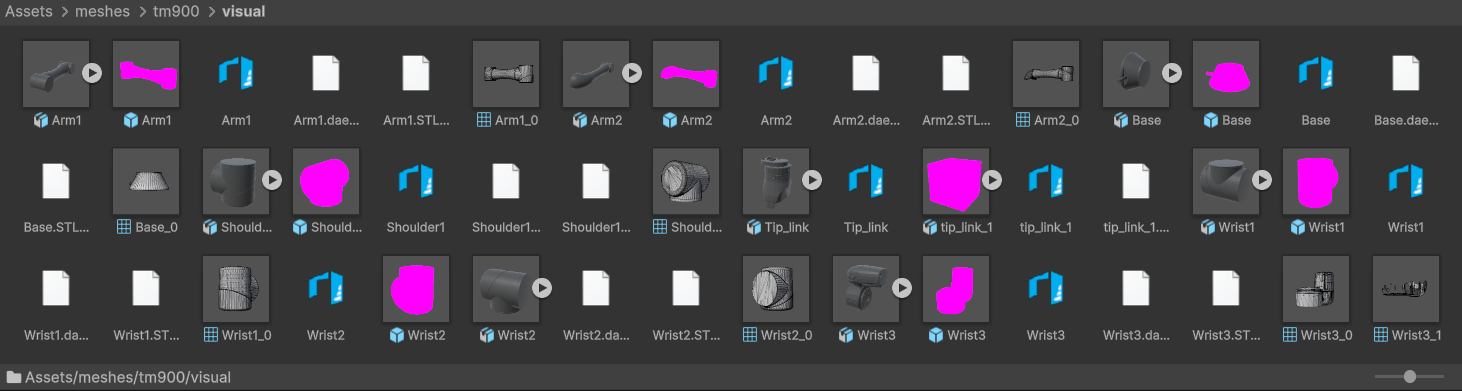
\includegraphics[width=0.8\textwidth]{images/prefab_visual.PNG}
    \caption{Cartella "visual" con i file .prefab generati automaticamente da Unity}
    \label{fig:visual_prefab}
\end{figure}

\begin{figure} [H]
    \centering
    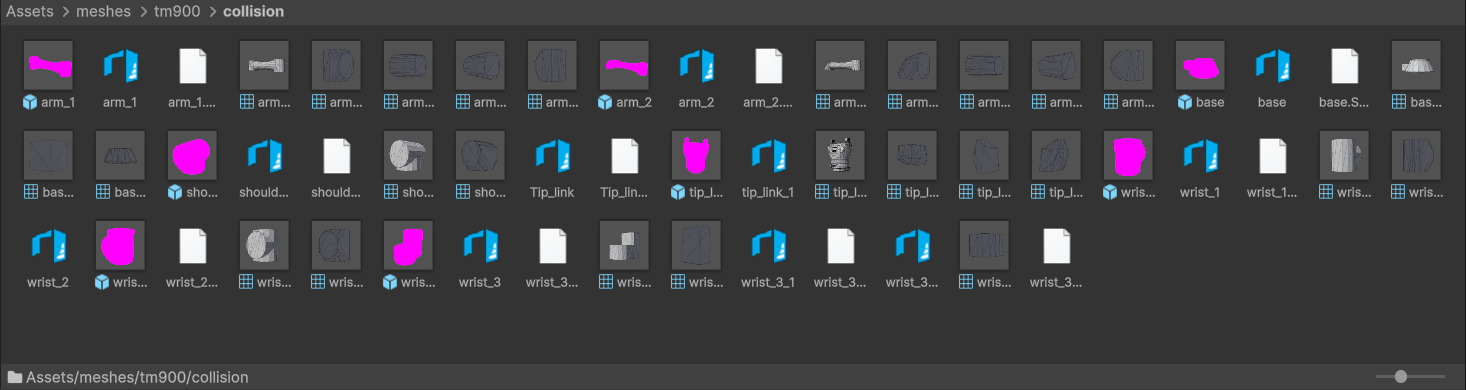
\includegraphics[width=0.8\textwidth]{images/prefab_collision.PNG}
    \caption{Cartella "collision" con i file .prefab generati automaticamente da Unity}
    \label{fig:collision_prefab}
\end{figure}

Tuttavia, una volta che il robot veniva cancellato dalla scena e quindi lo si voleva reimportare questi file .prefab venivano sovrascritti e il robot non veniva più visualizzato correttamente. In particolare, in fase di importazione l'errore che si otteneva era il seguente:

\begin{figure} [H]
    \centering
    
\includegraphics[width=1\textwidth]{images/errore_prefab.PNG}
    \caption{Errore durante l'importazione del file URDF del robot TM5-900}
    \label{fig:errore_prefab}
\end{figure}

Questo problema è stato risolto semplicemente eliminando i vari file .prefab all'interno della cartella "meshes" (sia in "visual" che in "collision").


\section{Problemi di visualizzazione delle meshes in Gazebo e Unity}
\label{sec:visualizzazione_meshes}
In questo progetto, sia su Gazebo che su Unity, si è utilizzato il file URDF per importare il robot TM5-900. Tuttavia, i due ambienti presentano differenze significative nell’interpretazione dei percorsi dei file che possono causare disallineamenti nella visualizzazione degli asset.
Quella che segue è una soluzione pratica a un problema avvenuto durante l'importazione del file URDF del robot in Gazebo e Unity.

\subsection{Problemi di visualizzazione delle meshes in Gazebo}
Come già proposto nella sezione \ref{sec:Importazione_TM5-900_Gazebo}, è possibile importare il robot TM5-900 utilizzando il file URDF. Tuttavia, durante il caricamento del file in Gazebo, si è riscontrato un errore di visualizzazione delle meshes, che non venivano caricate correttamente. Questo problema è stato causato da un errore nei percorsi delle meshes all'interno del file URDF. In particolare, i percorsi delle meshes erano stati definiti in questo modo:

\begin{verbatim}
    <link name="base_link">
    <visual>
      <geometry>
        <mesh filename="package://tm_description/meshes/tm900/visual/Base.STL"/>
      </geometry>
      <material name="Grey">
        <color rgba="0.5 0.5 0.5 1.0"/>
      </material>
    </visual>
    <collision>
      <geometry>
        <mesh filename="package://tm_description/meshes/tm900/collision/base.STL"/>
      </geometry>
    </collision>
    <inertial>
      <mass value="1.0"/>
      <insert_block name="origin"/>
      <inertia ixx="0.00110833289" ixy="0.0" ixz="0.0" iyy="0.00110833289" iyz="0.0" izz="0.0018"/>
    </inertial>
  </link>
\end{verbatim}

tuttavia Gazebo non riusciva a riconoscere il path, così la soluzione è stata quella di inserire il path completo a partire dalla cartella "home" di Linux, come mostrato di seguito:
\begin{verbatim}
    <link name="base_link">
    <visual>
      <geometry>
        <mesh filename="/home/User/ros2_workspace/install/tm_description/share/tm_description/meshes/tm900/visual/Base.STL"/>
      </geometry>
      <material name="Grey">
        <color rgba="0.5 0.5 0.5 1.0"/>
      </material>
    </visual>
    <collision>
      <geometry>
        <mesh filename="/home/User/ros2_workspace/install/tm_description/share/tm_description/meshes/tm900/collision/base.STL"/>
      </geometry>
    </collision>
    <inertial>
      <mass value="1.0"/>
      <insert_block name="origin"/>
      <inertia ixx="0.00110833289" ixy="0.0" ixz="0.0" iyy="0.00110833289" iyz="0.0" izz="0.0018"/>
    </inertial>
  </link>
\end{verbatim}
\subsection{Problemi di visualizzazione delle meshes in Unity}
Analogamente si è riscontrato un problema di visualizzazione delle meshes in Unity, dove il robot non veniva caricato correttamente. Anche in questo caso, il problema era dovuto a un errore nei percorsi delle meshes all'interno del file URDF. La soluzione è stata quella di modificare i percorsi delle meshes nel file URDF come mostrato di seguito:

\begin{verbatim}
    <link name="base_link">
    <visual>
      <geometry>
        <mesh filename="package://meshes/tm900/collision/base.STL"/>
      </geometry>
      <material name="Grey">
        <color rgba="0.5 0.5 0.5 1.0"/>
      </material>
    </visual>
    <collision>
      <geometry>
        <mesh filename="package://meshes/tm900/collision/base.STL"/>
      </geometry>
    </collision>
    <inertial>
      <mass value="1.0"/>
      <insert_block name="origin"/>
      <inertia ixx="0.00110833289" ixy="0.0" ixz="0.0" iyy="0.00110833289" iyz="0.0" izz="0.0018"/>
    </inertial>
  </link>
\end{verbatim}

facendo attenzione a inserire nella cartella Assets di Unity la prima cartella definita dopo "package://", in questo caso "meshes". In questo modo Unity riesce a riconoscere il path e caricare correttamente le meshes del robot.
\chapter{Struttura del workspace ROS2}
\textit{In questo capitolo viene presentata la struttura del workspace ROS2, con particolare attenzione alla disposizione dei pacchetti e dei file necessari per l'integrazione con Unity e la simulazione del robot. Come sotto riportato, i package sono evidenziati in rosso mentre i file Python sono evidenziati in blu.}

\begin{Verbatim}[commandchars=\\\{\}]
Dynamics/
    |-- ros2_humble/
    |   |-- src/
    |   |   |-- \textcolor{red}{moveit_config_tm5_900/}
    |   |   |   |-- config/
    |   |   |   |-- launch/
    |   |   |   |   |-- \textcolor{blue}{demo.launch.py}
    |   |   |   |   |-- \textcolor{blue}{move_group.launch.py}
    |   |   |   |   |-- \textcolor{blue}{setup_assistant.launch.py}
    |   |   |   |-- .setup_assistant
    |   |   |   |-- CMakeLists.txt
    |   |   |   `-- package.xml
    |   |   |-- \textcolor{red}{my_ros2_package/}
    |   |   |   |-- my_ros2_package/
    |   |   |   |   |-- build/
    |   |   |   |   |-- install/ 
    |   |   |   |   |-- log/
    |   |   |   |   |-- \textcolor{blue}{moveit_controller.py}
    |   |   |   |   `-- \textcolor{blue}{pose_listener.py}  
    |   |   |   |-- resource/
    |   |   |   |-- test/
    |   |   |   |-- setup.cfg
    |   |   |   `-- setup.py
    |   |   |-- \textcolor{red}{tm_description/}
    |   |   |   |-- config/
    |   |   |   |-- launch/  
    |   |   |   |-- meshes/
    |   |   |   |-- urdf/
    |   |   |   |-- CMakeLists.txt
    |   |   |   |-- package.xml
    |   |   `-- \textcolor{red}{tm_moveit_config/}
    |   |       |-- ...
    |   |-- install/
    |   |-- build/
    |   `-- log/
\end{Verbatim}

\newpage

Nel diagramma sono state riportate solo le cartelle e i file considerati più rilevanti per la comprensione dell'architettura del workspace; la repository completa è disponibile a \cite{Repository_ROS2}.

Si segnala, inoltre, che il package \textcolor{red}{\texttt{tm\_moveit\_config}} non è stato ulteriormente implementato, in quanto è stato creato automaticamente tramite il MoveIt Setup Assistant e presenta la stessa struttura di \textcolor{red}{\texttt{moveit\_config\_tm5\_900}}, spiegata nel dettaglio alla sezione \ref{sec:moveit}.

Questi due package influenzano direttamente il funzionamento del robot e sono stati creati per gestire la cinematica e la dinamica del braccio robotico. Tramite il comando 
\begin{verbatim}
    ros2 launch moveit_config_tm5_900 setup_assistant.launch.py
\end{verbatim}
oppure
\begin{verbatim}
    ros2 launch tm_moveit_config setup_assistant.launch.py
\end{verbatim} 
per i due package, si avvierà il Moveit Setup Assistant con il quale è possibile variare le pose del robot, le traiettorie e i giunti influenzati da esse. Il file \textcolor{blue}{\texttt{demo.launch.py}} permette di avviare il MoveIt2 demo, che consente di testare le funzionalità del robot in un ambiente simulato (approfondimento alla sezione \ref{sec:moveit}). Il file \textcolor{blue}{\texttt{move\_group.launch.py}} è il nodo principale che gestisce la comunicazione tra ROS2 e MoveIt2, mentre il file \textcolor{blue}{\texttt{setup\_assistant.launch.py}}, come già accenato, è utilizzato per configurare il robot e le sue proprietà cinematiche.
\newline
La cartella \textcolor{red}{\texttt{my\_ros2\_package}} contiene gli script Python che, una volta stabilita la connessione e avviati i controllori di Moveit, inviano i comandi da ROS2 a Unity, in particolare il file \textcolor{red}{\texttt{moveit\_controller.py}} che si occupa di simulare la movimentazione del robot TM5-900 in Unity dalla posa di "Home" a quella di "Work" definite nel Moveit Setup Assistant. Questo file è fondamentale per l'integrazione tra ROS2 e Unity, in quanto consente di controllare il robot direttamente dall'interfaccia grafica di Unity, facilitando la simulazione e il test delle traiettorie.
\newline
La cartella \textcolor{red}{\texttt{tm\_description}} contiene i file URDF e i modelli 3D necessari per rappresentare il robot in Gazebo e Unity. In questo package è importante che siano presenti le meshes all'interno della cartella \texttt{meshes}, sia di visualizzazione che di collisione, e il file URDF all'interno della cartella \texttt{urdf}.
In particolare il file URDF è possibile generarlo a partire dal file xacro tramite il comando:
\begin{verbatim}
    ros2 run xacro xacro nome_file.xacro > nome_file.urdf
\end{verbatim}
Il file URDF è fondamentale per la rappresentazione del robot in Gazebo e Unity, in quanto definisce la struttura e le proprietà fisiche del robot, inclusi i link, i giunti e le collisioni. Inoltre, il file URDF deve essere correttamente configurato per garantire che il robot venga visualizzato e simulato correttamente in entrambi gli ambienti e quindi che i path relativi alle meshes siano corretti (problematiche riguardo ai path delle meshes nei vari software alla sezione \ref{sec:visualizzazione_meshes}).

\chapter{Test Effettuati e Risultati Ottenuti}
\label{cap:Test}
\textit{In questo capitolo si vuole guidare il lettore attraverso i test effettuati e i risultati ottenuti durante lo sviluppo del progetto. I test sono stati suddivisi in tre sezioni principali: test di comunicazione tra ROS2 e Unity, test di simulazione del movimento del robot in Unity e test di integrazione della camera. Ogni sezione presenta una descrizione dettagliata dei test effettuati, dei risultati ottenuti e delle eventuali problematiche riscontrate.}

\section{Test di comunicazione tra ROS2 e Unity}
\label{sec:Test_comunicazione}

\section{Test di simulazione del movimento del robot in Unity}
\label{sec:Test_simulazione}    

\section{Test di integrazione della camera}
\label{sec:Test_camera} 


\chapter{Conclusioni}
\label{cap:Conclusioni}
\section{Applicazione finale}
% Nell'introduzione al capitolo specificate anche la versione dell'STM32CubeIDE e dell'STM32CubeMX che avete usato (se avete cambiato versione nel corso del progetto mettete l'ultima, quella su cui è sviluppato il codice che consegnate).

% \section{Diagramma di flusso}
% Inserire un diagramma di flusso analogo a quello in Figura \ref{fig:diagramma} che spiega il funzionamento generale del codice sviluppato. Inserire anche una descrizione testuale del funzionamento.

% \begin{figure}[H]
% \centering
% 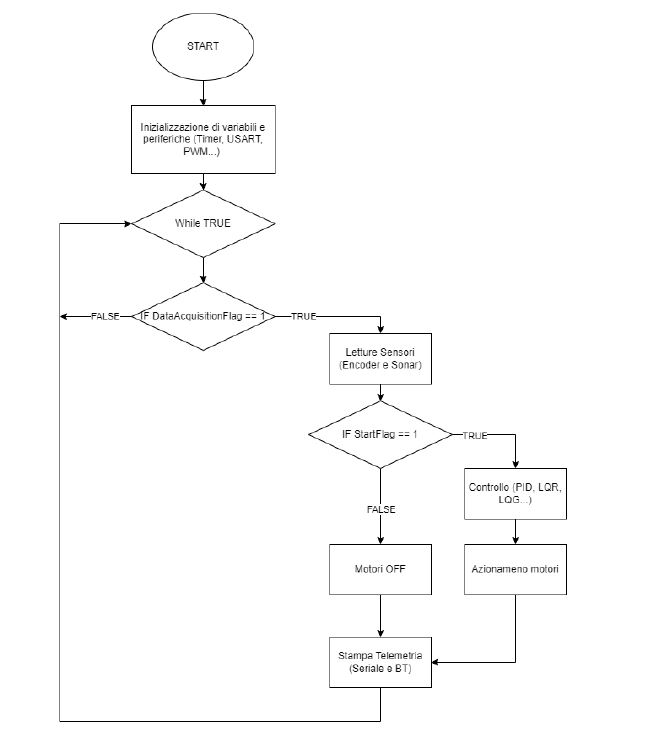
\includegraphics[width=0.8\textwidth,keepaspectratio]{figures/diagramma.JPG}
% \caption{Diagramma di flusso del codice sviluppato}
% \label{fig:diagramma}
% \end{figure}

% \section{Gestione singoli componenti}
% Dedicare un pagagrafo ad ogni componente in cui viene spiegato il codice che lo gestisce. Inserite prima una descrizione generale di come si gestisce un componente di quel tipo (aiutandovi con schemi o altro). Poi le configurazioni che sono state fatte sul .ioc per poterlo utilizzare (quale periferiche sono state abilitate, come sono state configurate.. mettete degli screen del .ioc). Infine inserite e spiegate le parti di codice che lo gestiscono.\\
% \newline
% \textcolor{red}{NOTA per il codice}: per rendere il codice modulare e riutilizzabile è buona prassi non caricare troppo il main ma creare una libreria per ogni componente. Quindi il componente1 avrà un header file "componente1.h" e un source file "componente1.c", nel source file sono implementate le funzioni che gestiscono il componente, nell'header file ci sono i prototipi di tali funzioni in modo che esse possano essere usate nel main includendolo.\\
% \newline
% \textcolor{red}{NOTA per il codice}: non inserire mai nel codice dei parametri numerici senza contesto ma renderli delle costanti definite (usando la direttiva \%define). Se sono delle costanti relative ad uno specifico componente vanno inserite nel relativo header file.\\
% \newline
% \textcolor{red}{NOTA per il codice}: per inserire il codice, anziché utilizzare screenshot utilizzate i seguenti comandi.\\
% Per codice scritto in latex (con linguaggio Python):
% \begin{lstlisting}[language=Python, caption="Codice in Python"]
% import numpy as np
    
% def incmatrix(genl1,genl2):
%     m = len(genl1) # The length of the first array
%     n = len(genl2) # The length of the second array
%     sum = 0
    
%     # Compute 
%     for i in range(0,n):
%         for j in range(0, m):
%             sum += genl1[n]*genl2[m]

%     # Print
%     print("The sum is %2d" %(sum))   
    
%     return M
% \end{lstlisting}
% Per codice richiamato da file (con linguaggio C):

% \lstinputlisting[language=Cpp, firstline=4, lastline=8, caption="Codice in C"]{codefiles/example_code.cpp}

% Funziona anche per codice MATLAB:
% \begin{lstlisting}[language=MATLABc, caption="Codice in MATLAB"]
% %% PREPARE WORKSPACE
% close all
% clearvars
% clc

% %% OPERATIONS
% sayhello;

% %% FUNCTIONS
% function sayhello
%     fprintf("Hello world!");
% end

% \end{lstlisting}


% \subsection{Gestione componente1}

% \subsection{Gestione componente2}

% \section{Funzionamento complessivo}
% Dopo aver spiegato il codice che gestisce i singoli componenti, inserire e commentare le porzioni di codice relative al funzionamento complessivo del programma.

% Dedicate un capitolo a tutti i test effettuati con relativi risultati, includete sia i test finali relativi al funzionamento complessivo, sia i test delle singole parti (se significativi). \\
% Descrivete in dettaglio le condizioni in cui sono stati svolti i test in modo che siano ripetibili. Durante i test fate dei video e acquisite i dati (es usando la funzione di log di Putty), per i test più rilevanti è opportuno consegnare anche questo materiale per documentare i test effettuati. Nella relazione riportate i risultati con dei grafici come quello in Figura \ref{fig:grafico} (inserite sempre nei grafici le label sugli assi con grandezza e relativa unità di misura). Commentate in modo critico i risultati ottenuti, evidenziando sia quelli positivi sia quelli negativi. 

% \begin{figure}[H]
% \centering
% 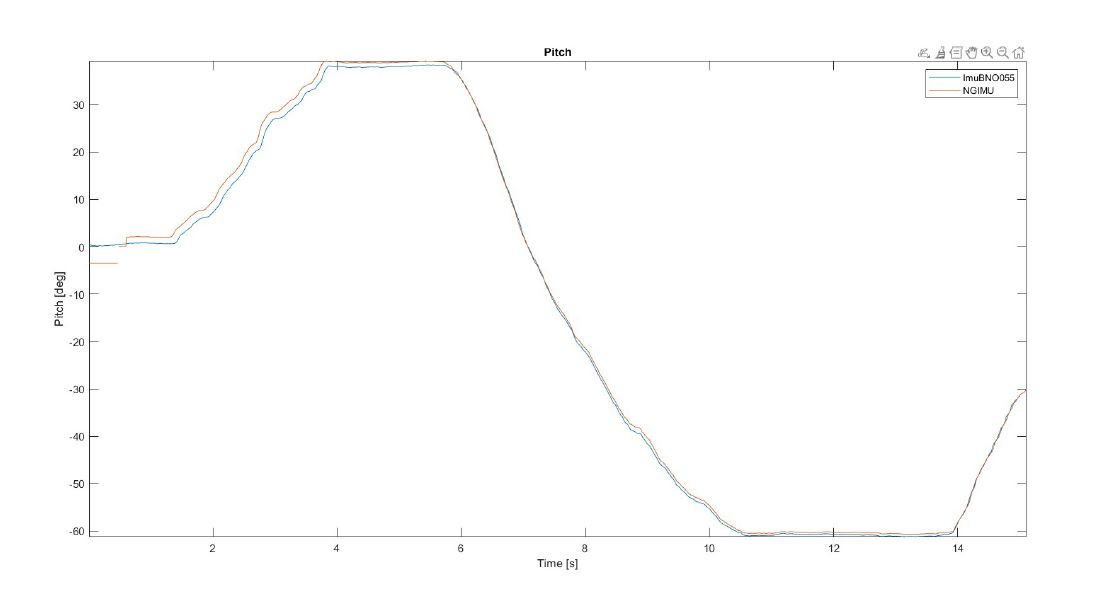
\includegraphics[width=0.8\textwidth,keepaspectratio]{figures/grafico.JPG}
% \caption{Esempio di grafico}
% \label{fig:grafico}
% \end{figure}
% \section{Test1}
% Per ogni test riportate: cosa state testando, in che condizioni si è svolto il test, riferimenti a video/file di log che consegnate insieme a relazione e codice, grafici dei risultati, commento dei risultati.

% \section{Test2}

% \newpage
% \addcontentsline{toc}{chapter}{Conclusioni e sviluppi futuri}
% \section*{Conclusioni e sviluppi futuri}
% Riassumere brevemente il lavoro svolto rispetto al task assegnato, evidenziando quali risultati sono stati raggiunti e quali no. Se ci sono aspetti del task non completati spiegare quali sono stati i problemi riscontrati in merito.\\
% Inserire considerazioni personali su possibili sviluppi futuri dell'attività svolta (idee per migliorarla che non avete avuto modo di sperimentare, aspetti che suggerite di approfondire, problemi da risolvere..).

\addcontentsline{toc}{chapter}{Appendici}
\appendix
\chapter{Appendice1}
Se necessario ricorrete alle appendici per spiegare le parti "di contorno" dell'attività svolta e/o ciò che non riuscite ad inserire nello schema generale dei capitoli della relazione (es acquisizione dei dati con Matlab).


\bibliographystyle{ieeetr}
\bibliography{bibl} 

\end{document}
